% CVPR 2026 Paper Template; see https://github.com/cvpr-org/author-kit

\documentclass[10pt,twocolumn,letterpaper]{article}

%%%%%%%%% PAPER TYPE  - PLEASE UPDATE FOR FINAL VERSION
% \usepackage{cvpr}              % To produce the CAMERA-READY version
% \usepackage[review]{cvpr}      % To produce the REVIEW version
\usepackage[pagenumbers]{cvpr} % To force page numbers, e.g. for an arXiv version

\usepackage[accsupp]{axessibility}  % Improves PDF readability for those with disabilities.

% Import additional packages in the preamble file, before hyperref
\input{preamble}

% It is strongly recommended to use hyperref, especially for the review version.
% hyperref with option pagebackref eases the reviewers' job.
% Please disable hyperref *only* if you encounter grave issues, 
% e.g. with the file validation for the camera-ready version.
%
% If you comment hyperref and then uncomment it, you should delete *.aux before re-running LaTeX.
% (Or just hit 'q' on the first LaTeX run, let it finish, and you should be clear).
\definecolor{cvprblue}{rgb}{0.21,0.49,0.74}
\usepackage[pagebackref,breaklinks,colorlinks,allcolors=cvprblue]{hyperref}

\newcommand\sss[1]{\textcolor{purple}{[\textbf{ss}: #1]}}

%%%%%%%%% PAPER ID  - PLEASE UPDATE
\def\paperID{} % *** Enter the Paper ID here
\def\confName{CVPR}
\def\confYear{2026}

%%%%%%%%% TITLE - PLEASE UPDATE
% \title{GeoPredict: A Vision-Language-Action Framework with \underline{Predict}ive Kinematic and \underline{Geo}metric Priors}
% \title{GeoPredict: Predictive Kinematic and 3D Geometric Priors for Vision–Language–Action Manipulation}
\title{GeoPredict: Leveraging Predictive Kinematics and 3D Gaussian Geometry for Precise VLA Manipulation}

%%%%%%%%% AUTHORS - PLEASE UPDATE
\author{
    Jingjing Qian$^{1}$ \quad
    Boyao Han$^{2}$ \quad
    Chen Shi$^{1}$ \quad
    Lei Xiao$^{1}$ \quad
    Long Yang$^{1}$ \quad
    Shaoshuai Shi$^{3}$ \quad
    Li Jiang$^{1\dagger}$ \\
    $^{1}$The Chinese University of Hong Kong, Shenzhen \\
    $^{2}$Hunan University \quad
    $^{3}$Voyager Research, Didi Chuxing \\[5pt]
    {\tt\small \url{https://jingjingqian75.github.io/GeoPredict-Page/}}
}







\begin{document}
\maketitle
{
    \renewcommand{\thefootnote}{$\dagger$}
    \footnotetext{Corresponding Author.}
}
\begin{abstract}
Vision--Language--Action (VLA) models achieve strong generalization in robotic manipulation but remain largely reactive and 2D-centric, making them unreliable in tasks that require precise 3D reasoning. We propose \textbf{GeoPredict}, a geometry-aware VLA framework that augments a continuous-action policy with predictive kinematic and geometric priors. GeoPredict introduces a trajectory-level module that encodes motion history and predicts multi-step 3D keypoint trajectories of robot arms, and a predictive 3D Gaussian geometry module that forecasts workspace geometry with track-guided refinement along future keypoint trajectories. These predictive modules serve exclusively as training-time supervision through depth-based rendering, while inference requires only lightweight additional query tokens without invoking any 3D decoding. Experiments on RoboCasa Human-50, LIBERO, and real-world manipulation tasks show that GeoPredict consistently outperforms strong VLA baselines, especially in geometry-intensive and spatially demanding scenarios.


\end{abstract}    
\section{Introduction}
\label{sec:intro}

% Vision--Language--Action (VLA) models have recently emerged as a promising paradigm for robotic manipulation, leveraging large pre-trained Vision--Language Models (VLMs) to map rich visual observations and language instructions directly to actions~\cite{kim2025openvla,black2410pi0}. By inheriting semantic and visual priors from internet-scale data, these models exhibit strong generalization across diverse tasks and environments. However, most VLAs reason primarily in 2D image space and generate actions reactively from the current observation, without anticipating how robot motion will alter the underlying 3D scene. This 2D-centric and myopic formulation limits performance in manipulation tasks that require precise spatial reasoning, object-centric geometry understanding, and physically consistent long-horizon behavior.

% A natural direction is to augment policies with a \emph{world model} capable of predicting future environment states~\cite{lu2025gwm,cen2025worldvla}. Early world models emphasized latent dynamics for planning or reinforcement learning, but these lacked the explicit geometry needed for contact-rich manipulation. More recent approaches predict future RGB frames or point-based representations~\cite{hu2025videopredictionpolicy,liu2025geometryaware4d}, yet such view-dependent predictions struggle with multi-view consistency and do not provide the structured 3D scene information required to reason about object poses or end-effector clearances. Moreover, tightly coupling a high-capacity world model with a large VLA backbone can quickly become computationally prohibitive, especially if multi-view 3D prediction is required at inference time.

% For effective visuomotor control, we argue that two predictive capabilities are particularly valuable. First, the policy should leverage \emph{predictive kinematic priors} describing how the robot is likely to move over the next several steps, rather than relying solely on instantaneous joint states. Second, it should reason about \emph{predictive 3D scene geometry} through an explicit, differentiable representation that can be supervised using depth and multi-view signals. Crucially, such predictive signals must integrate seamlessly with VLA models while preserving deployment efficiency.


Vision--Language--Action (VLA) models have recently emerged as a powerful paradigm for robotic manipulation, leveraging large pre-trained Vision--Language Models (VLMs) to map rich visual observations and language instructions directly to actions~\cite{brohan2022rt, zitkovich2023rt, li2024cogact, zheng2025universal}. By inheriting semantic and visual priors from internet-scale data, these models generalize well across tasks and settings. However, they operate primarily in 2D image space, mapping the current observation reactively and lacking explicit 3D spatial modeling~\cite{zhong2025survey}. This 2D-centric, myopic formulation limits performance in tasks requiring precise 3D reasoning and physically consistent long-horizon control.

To move beyond purely reactive policies, recent work has begun to incorporate predictive structure into visuomotor models~\cite{hu2025video, li2025unified, lu2025gwm}. Some approaches learn latent dynamics or temporal abstractions to better capture how states evolve over time~\cite{chen2025villa, chen2025moto, li2024vision, zhao2025cot}, while others predict future observations such as RGB frames, depths, or point-based representations~\cite{cen2025worldvla,zhangdreamvla,hu2025video,qian2025wristworld, grauman2022ego4d,gupta2024pre}. Although these methods provide useful temporal signals, they often remain view-independent and do not strictly enforce multi-view or 3D geometric consistency, making it hard to reason about object poses, clearances, and end-effector motion in workspace coordinates. Moreover, tightly coupling high-capacity predictive modules with large VLA backbones can introduce non-negligible computational overhead if complex 3D prediction is required during inference time.

For robotic manipulation, we argue that two predictive capabilities are particularly valuable. First, the policy should exploit \emph{predictive kinematic priors} that summarize how the robot is likely to move over the next few steps, rather than relying solely on instantaneous joint states. Second, it should reason about \emph{predictive 3D Gaussian geometry} through an explicit, differentiable representation aligned with the robot’s workspace and amenable to supervision from depth and multi-view cues. Crucially, these predictive signals must seamlessly integrate with VLA architectures and keep inference-time overhead modest enough to enable practical deployment for real-time robotic control.

In this paper, we introduce \textbf{GeoPredict}, a geometry-aware VLA framework augmented with predictive priors for robotic manipulation. GeoPredict is built on top of a strong continuous-action VLA policy~\cite{black2410pi0}, and augments the policy with two complementary predictive modules.

First, at the kinematic level, we introduce a \emph{trajectory-level prediction module} that tracks key robot joints and end-effector points and encodes their motion history into compact tokens via a Track Encoder. A set of learnable future track queries then predicts multi-step 3D keypoint trajectories, providing explicit, differentiable kinematic priors. These predicted trajectories not only regularize the transformer's internal dynamics, but also serve as guidance for where high-fidelity 3D scene modeling is most needed.

Second, at the geometric level, we introduce a \emph{predictive 3D Gaussian geometry module} that forecasts how workspace geometry evolves over time. A coarse 3D spatial query grid is decoded into Gaussian primitives representing the scene at future timesteps. To focus geometric capacity where precision matters most, a track-guided refinement mechanism increases Gaussian density along the predicted future keypoint trajectories of the joints, yielding higher resolution around anticipated motion and interaction regions. The resulting 3DGS representation is supervised through future depth-map rendering, providing a geometry-focused training signal without requiring color modeling.

Both predictive modules are integrated via a block-wise causal attention hierarchy and are used only during training; inference behaves exactly like the base VLA policy.

In summary, our main contributions are threefold:
(1) We introduce \textbf{GeoPredict}, a geometry-aware VLA framework that injects future-aware kinematic and geometric priors into a continuous-action VLA policy, enhancing reasoning about long-horizon 3D dynamics.
(2) We propose two complementary predictive modules: a trajectory-level kinematic predictor forecasting multi-step robot keypoint motion, and a predictive 3D Gaussian geometry module with track-guided refinement that allocates geometric capacity to task-relevant interaction regions.
(3) We show that GeoPredict delivers consistent and substantial improvements over strong VLA baselines on RoboCasa Human-50, LIBERO, and real-world manipulation tasks, particularly those requiring precise spatial reasoning and geometric robustness.

\section{Related Work} \label{sec:related_work}

\subsection{Vision-Language-Action Models}

Vision-Language-Action (VLA) models have emerged as powerful robotic policies~\cite{brohan2022rt, kim2025openvla, li2024cogact, zheng2024tracevla, zheng2025universal, xiao2025ava}. Pioneering methods like OpenVLA~\cite{kim2025openvla} rely on discrete autoregressive tokenization, limiting inference frequency and struggling with continuous, multi-modal action distributions~\cite{zhong2025survey}. While subsequent architectures like $\pi_0$~\cite{black2410pi0} utilize conditional flow matching~\cite{lipman2022flow} to generate continuous actions, they remain predominantly 2D-centric and reactive~\cite{bu2025univla, black2410pi0, hu2025video, zheng2024tracevla}, lacking the robust 3D geometric understanding required for complex manipulation. Furthermore, although SpatialVLA~\cite{qu2025spatialvla} and BridgeVLA~\cite{li2025bridgevla} integrate explicit 3D information and auxiliary tasks, they still lack a predictive understanding of 3D scene dynamics. To address this gap, our GeoPredict introduces a geometry-aware predictive model that directly forecasts 3D scene evolution using 3D Gaussian Splatting~\cite{kerbl20233d}, equipping the VLA model with predictive geometric priors.



\subsection{Future Prediction for Robotic Manipulation}

Recent works explore future prediction to enhance robotic policies~\cite{cen2025worldvla, zhang2023storm, hafnermastering, micheli2022transformers, hansen2023td, hafner2022deep}. Some directly forecast future observations like RGB images~\cite{wu2024unleashing, hu2025video}, depths~\cite{zhangdreamvla}, or pointmaps~\cite{liu2025geometry}, while approaches like Seer~\cite{tianpredictive} condition inverse dynamics on these forecasted visual states. However, these methods face two key limitations. First, popular approaches like SuSiE~\cite{black2023zero} or UniPi~\cite{du2023learning} often rely on a single prediction step, which struggles to capture complex physical dynamics and introduces time-consuming denoising that reduces control frequency. Second, these 2D-centric methods~\cite{wu2024unleashing} struggle with multi-view consistency and lack the explicit 3D geometry crucial for accurate manipulation. To address this gap, we introduce GeoPredict, a geometry-aware predictive model that forecasts scene evolution over a full horizon of $H$ steps in explicit 3D space, learning a spatially coherent and predictive 3D representation to condition action generations.



\subsection{3D Scene Representation} 

3D scene representation is a fundamental problem in computer vision, traditionally relying on explicit structures like meshes~\cite{lorensen1998marching}, voxels~\cite{wu20153d} and point clouds~\cite{qi2017pointnet}. Recent research has shifted to neural representations that learn continuous models of scene geometry and appearance. Pioneered by Neural Radiance Fields (NeRF)~\cite{mildenhall2021nerf}, these implicit models often require subsequent acceleration~\cite{muller2022instant,xu2022point,hu2022efficientnerf} due to costly training and rendering. More recently, 3D Gaussian Splatting (3DGS)~\cite{kerbl20233d,yan2024street,wu20244d,ren2024scube} has emerged as a highly effective explicit alternative. 3DGS models scenes as a collection of 3D Gaussians with learned attributes, leveraging differentiable rasterization for high-fidelity and remarkably efficient rendering. While recent works like GWM~\cite{lu2025gwm} apply 3DGS to robotic world modeling, directly forecasting these massive Gaussian attributes remains computationally demanding. To circumvent this burden, we leverage 3DGS as a predictive scene geometry module solely during training, aiming to endow the VLA policy with intrinsic, foresight-driven spatial reasoning ability.

\section{Methodology}
\label{sec:method}

\begin{figure*}[htbp]
  \centering
  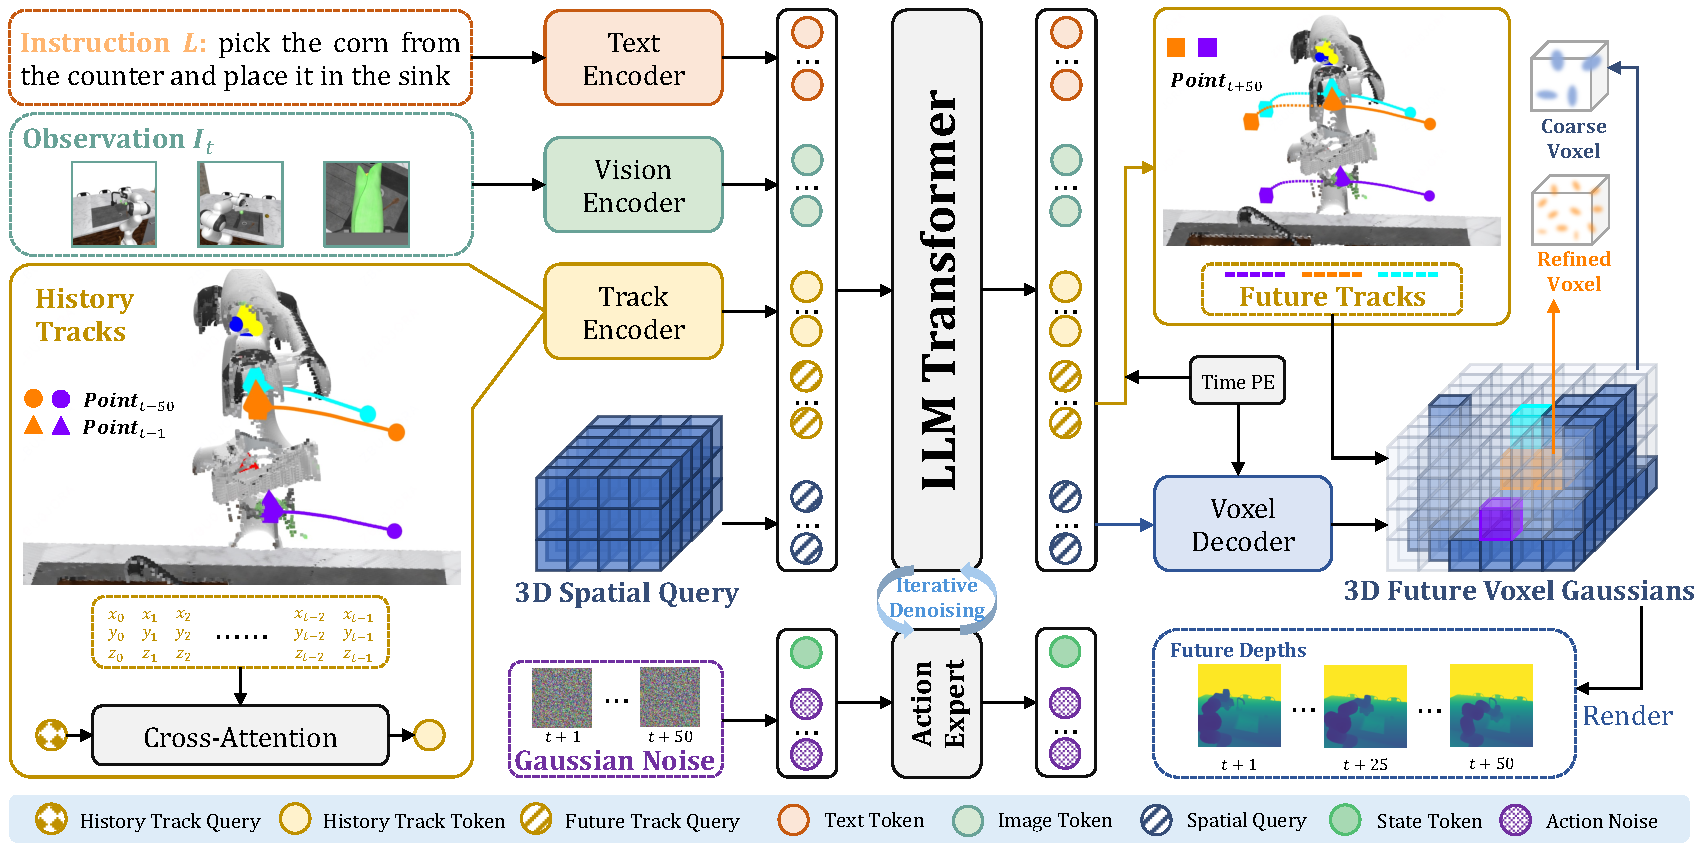
\includegraphics[width=0.99\textwidth]{fig/method.pdf}
  \caption{\textbf{Overview of GeoPredict.} Given an instruction, multi-view images and motion history encoded by the Track Encoder, a central LLM Transformer learns two main tasks. First, it predicts multi-timestep 3D keypoint trajectories using learnable Future Track Query. Second, it forecasts future workspace geometry as a predictive 3D Gaussian by processing a 3D Spatial Query through a Voxel Decoder. A track-guided refinement mechanism leverages the predicted future tracks to allocate geometric capacity to task-relevant interaction regions. Our policy then generates the final action via an Action Expert. Crucially, these predictive modules serve exclusively as training-time supervision and are not invoked during inference, thus preserving efficiency.}
\label{fig:method}
\vspace{-15pt}
\end{figure*}

% 一段话简单介绍一下章节内容，结合图1给出方法的概况说明。

% Our objective is to endow a Vision-Language-Action (VLA) policy with \emph{predictive spatial intelligence}: before committing to low-level control, the policy should form expectations about how the robot and the scene will evolve. To this end, we propose \textbf{GeoPredict}, a training-time world-model-augmented VLA framework that couples (i) trajectory-level kinematic forecasting for robot keypoints with (ii) predictive 3D Gaussian Splatting (3DGS) for future scene geometry. These two sources of foresight are injected into a language-conditioned, flow-matching action head. Crucially, all heavy 3D prediction components are used only during training; at inference, the system retains the efficiency of the VLA backbone.

% We propose \textbf{GeoPredict}, a world-model-augmented Vision–Language–Action (VLA) framework that equips continuous control policies with predictive kinematic and geometric priors. GeoPredict jointly learns future robot keypoint trajectories and future scene geometry represented via 3D Gaussian Splatting (3DGS), and conditions the underlying VLA model on these predictive signals. Importantly, these predictive modules are applied only during training, while the action generation stage follows the standard VLA formulation.

% We first present the problem setup and the VLA model we build upon (Sec.~\ref{sec:preliminary}). We then describe our trajectory-encoding and prediction module (Sec.~\ref{sec:track_query}), followed by our predictive 3D world model and refinement strategy (Sec.~\ref{sec:3dgs}). Finally, we outline the attention design, training objective, and inference process (Sec.~\ref{sec:train_infer}).

We propose \textbf{GeoPredict}, a geometry-aware VLA framework that equips continuous-control policies with predictive kinematic and geometric priors. GeoPredict jointly learns future robot keypoint trajectories and future scene geometry through a 3DGS representation, and conditions the underlying VLA on these predictions. Notably, these predictive modules are used only during training, while the action generation process remains similar to a standard VLA policy.

First, we describe the problem setup and the base VLA model (Sec.~\ref{sec:preliminary}). We then introduce our trajectory encoding and future motion prediction module (Sec.~\ref{sec:track_query}), followed by the predictive 3D Gaussian geometry and its refinement mechanism (Sec.~\ref{sec:3dgs}). Finally, we present the attention design, training objective and inference process (Sec.~\ref{sec:train_infer}).


\subsection{Preliminary} \label{sec:preliminary}

\textbf{Problem Definition.}
%
% The VLA paradigm~\cite{kim2025openvla,black2410pi0} aims to learn a policy $\bm{\pi}$ that maps a language instruction $\textbf{L}$, current observation $\textbf{O}_t$, and robot proprioception $\textbf{Q}_t$ to a continuous action chunk $\textbf{A}_t=[\textbf{a}_t,\textbf{a}_{t+1},...,\textbf{a}_{t+H-1}]$ (we use $H=50$ in our method).
% Here, we use multi-view images $\mathbf{I}_t$ and joint coordinates $\mathbf{J}_t$ as $\mathbf{O}_t=(\mathbf{I}_t,\mathbf{J}_t)$. Each action $\mathbf{a}_t\in\mathbb{R}^{D}$ is a 7-DoF end-effector control vector
% $\mathbf{a}_t=\{\Delta\mathbf{x},\Delta\bm{\theta},g\}$, where $\Delta \bm{x} \in \mathbb{R}^3$ is the control translation, $\Delta \bm{\theta} \in \mathbb{R}^3$ is the rotation offset (e.g., axis-angle or Euler representation), and $g \in \mathbb{R}$ represents the gripper's open-close state.  
%
The VLA paradigm~\cite{kim2025openvla,black2410pi0} aims to learn a policy $\bm{\pi}$ that maps a language instruction $\mathbf{L}$, the current multi-view image observation $\mathbf{I}_t$, and the robot’s proprioceptive state $\mathbf{Q}_t$ to a continuous action chunk $\mathbf{A}_t=[\mathbf{a}_t, \mathbf{a}_{t+1}, \ldots, \mathbf{a}_{t+H-1}]$, where we set $H=50$. 
% The observation $\textbf{O}_t$ consists of multi-view images $\textbf{I}_t$ and joint coordinates $\textbf{J}_t$, i.e., $\textbf{O}_t=(\textbf{I}_t,\textbf{J}_t)$. 
Each action $\mathbf{a}_t \in \mathbf{R}^{7}$ is a 7-DoF end-effector command $\mathbf{a}_t=\{\Delta\mathbf{x}, \Delta\bm{\theta}, g\}$,
where $\Delta\mathbf{x}\in\mathbb{R}^3$ and $\Delta\bm{\theta}\in\mathbb{R}^3$ denote translational and rotational offsets (e.g., in axis–angle or Euler representation), and $g\in\mathbb{R}$ is the gripper's open-close state.

% Traditional VLAs typically predict actions reactively from current observations. However, many manipulation tasks fundamentally require anticipating how the robot and the environment will change\sss{CHECK}. GeoPredict therefore conditions the policy not only on past observations but also on internally generated predictions of future motion and future scene geometry.

While  VLAs generate actions reactively from the current observation, many manipulation tasks require anticipating how both the robot and the surrounding scene will evolve over time. Thus, GeoPredict augments the policy by conditioning not only on past observations but also on internally predicted future robot motion and future scene geometry.

%
% The standard paradigm for Vision-Language-Action (VLA) models~\cite{kim2025openvla, black2410pi0} aims to learn a policy $\bm{\pi}$ that maps a language instruction $\textbf{L}$, the current observation $\textbf{O}_t$ and the robot's proprioceptive state $\textbf{Q}_t$ to a continuous, low-level robot action chunk $\textbf{A}_t=[\textbf{a}_t,\textbf{a}_{t+1},...,\textbf{a}_{t+H-1}]$ (we use $H=50$ in our method). Here, the observation $\textbf{O}_t$ consists of multi-view images $\textbf{I}_t$ and the robot's joint coordinates $\textbf{J}_t$. The action $\textbf{a}_t \in \mathbb{R}^D$ defines the low-level control command, represented as a continuous vector $\textbf{a}_t = \{\Delta \bm{x}, \Delta \bm{\theta}, g\}$. This vector typically represents 7-DoF end-effector control, where $\Delta \bm{x} \in \mathbb{R}^3$ is the control translation, $\Delta \bm{\theta} \in \mathbb{R}^3$ is the rotation offset (e.g., axis-angle or Euler representation), and $g \in \mathbb{R}$ represents the gripper's open-close state. 
%
% Our model, GeoPredict, extends this basic definition by conditioning the policy  $\bm{\pi}$ not only on the past and present observations $\textbf{O}_{\leq t}$, but also on an internally generated \textit{prediction} of the future world state $\hat{\textbf{S}}_{t+k}$, which we formulate as a 3DGS world model.

\textbf{Base VLA model.}
We adopt $\pi_0$~\cite{black2410pi0} as the VLA base model. It comprises a VLM (PaliGemma~\cite{beyer2024paligemma} with a SigLIP vision encoder) and a robotics-specific \emph{action expert} that generates continuous actions via conditional flow matching~\cite{lipman2022flow}. Text, image, and proprioceptive tokens are projected into a shared space and processed by the transformer; the action expert then generates $\mathbf{A}_t$ by integrating a learned vector field from noise in a small, fixed number of steps.

% GeoPredict augments this base VLA model with predictive components that influence the transformer’s internal representations, without altering how actions are ultimately drawn from the action expert.



% \noindent \textbf{Vision-Language-Action Backbone.}
% We select $\pi_0$~\cite{black2410pi0} as our Vision-Language-Action (VLA) backbone. $\pi_0$ consists of a core VLM (PaliGemma~\cite{beyer2024paligemma}, which utilizes a SigLIP vision encoder and a Gemma transformer backbone) and is augmented with robotics-specific components. Following a standard late fusion VLM recipe, vision encoder processes multi-view images $\textbf{I}_t$ and embed them into the same embedding space as the language tokens derived from the text instruction $\textbf{L}$. The robot's proprioceptive state $\textbf{Q}_t$ is also projected into this common embedding space. These multimodal tokens are fed into the central LLM Transformer backbone. Critically, unlike prior VLAs that employ autoregressive discretization for actions~\cite{kim2025openvla, bu2025univla}, $\pi_0$ is augmented with a novel \textbf{action expert}, which utilizes a separate set of weights for robotics-specific tokens, generates continuous action distributions via \textbf{conditional flow matching}~\cite{lipman2022flow}. This process generates actions at inference time by starting with random noise and iteratively integrating a learned vector field over a fixed number of steps (e.g., 10 steps) to produce the final, denoised action chunk.


% \subsection{Track Encoder and Future Track Query} \label{sec:track_query}
\subsection{Trajectory-Level Kinematic Prediction} \label{sec:track_query}
% This section details the mechanisms for encoding historical motion and predicting future trajectories, which are essential for providing the model with kinematic priors and enabling predictive world modeling. We introduce a Track Encoder to compress past motion and a Future Track Query to generate future 3D point trajectories.


% GeoPredict first models robot motion at the trajectory level. This provides a compact summary of past kinematics and an explicit prediction of future keypoint trajectories, which act both as a kinematic prior for action generation and as guidance for spatial refinement in the 3D world model.

GeoPredict models robot motion at the trajectory level. This provides both a compact summary of past kinematics and an explicit prediction of future trajectories, serving as a kinematic prior for action generation and as guidance for spatial refinement in the following 3D Gaussian geometry module.



\noindent \textbf{Track Encoder.}
% The primary function of the Track Encoder is to distill the complete motion history of all relevant robot keypoints (joints and end-effectors) into a set of compact, fixed-dimensional tokens for consumption by the LLM Transformer. This historical context is critical because generating executable actions is fundamentally a task of predicting future trajectories. Given that joint movements possess inertia, these historical tokens provide a crucial kinematic prior, enabling the LLM to make physically plausible and informed predictions about future motion.
%
% The Track Encoder compresses the motion history of all robot keypoints into compact tokens for the transformer. This historical context serves as a kinematic prior: because joint motion exhibits inertia and action generation fundamentally involves forecasting trajectories, these tokens help the model make physically plausible and informed future motion predictions.
%
The Track Encoder compresses the motion history of all robot keypoints into compact tokens for the transformer. This historical context provides a strong kinematic prior: because joint motion exhibits inertia and action generation fundamentally involves forecasting future trajectories, encoding past dynamics enables the model to make more physically consistent motion predictions.


% As illustrated in Figure~\ref{fig:method}, we track $K$ 3D keypoints ($N$ joints and $M$ end-effectors, where $K=N+M$). For each keypoint $k$, we record its 3D coordinates from time $0$ to $t-1$ (visualized as $t-50$ to $t-1$ in Figure~\ref{fig:method} for brevity), forming a historical trajectory $\bm{\mathcal{T}}_k \in \mathbb{R}^{(t-1) \times 3}$. These $K$ trajectories are the inputs to the Track Encoder. Inside the encoder, we initialize a shared, learnable \textit{history track query} $\textbf{Q}^{hist}$. This query performs cross-attention with the embedded 3D coordinates of each trajectory $\bm{\mathcal{T}}_k$ to compress the entire variable-length temporal history of that keypoint into a single \textit{history track token} $\textbf{Z}_k^{hist}$. These $K$ tokens are then passed as input to the LLM Transformer. The cross-attention mechanism for generating the $k$-th token is formally defined as:
% \begin{equation}
% \begin{aligned}
% \mathbf{Z}_k^{hist} &= \text{CrossAttn}(\mathbf{Q}^{hist}, \bm{\mathcal{T}}_k) \\
% &= \text{Softmax}\left(\frac{\mathbf{Q}^{hist} \textbf{K}_k^T}{\sqrt{d_k}}\right) \textbf{V}_k,
% \end{aligned}
% \end{equation}
% where $\textbf{K}_k = \textbf{V}_k = \text{Embed}( \bm{\mathcal{T}}_k)$ are the key and value matrices derived from the embedded points, and $\mathbf{Q}^{hist}$ serves as the query. $d_k$ is the dimension of the key vector.

% As illustrated in Figure~\ref{fig:method}, we track $K$ 3D keypoints (joints and end-effector points). 
% For each keypoint $k\in\{1, ..., K\}$, we collect its 3D coordinates from time $0$ to $t-1$ into a trajectory $\bm{\mathcal{T}}_k \in \mathbb{R}^{(t-1) \times 3}$. 
% %
% A shared, learnable history query $\textbf{Q}^{hist}$ performs cross-attention over the embedded trajectory to compress it into a single token as:
% \begin{equation}
% \begin{aligned}
% \mathbf{Z}_k^{hist} = \text{CrossAttn}(&\text{query}=\mathbf{Q}^{hist},
% \text{key}= \text{MLP}(\bm{\mathcal{T}}_k),\\ &\text{value}=\text{MLP}(\bm{\mathcal{T}}_k)), \\
% % &= \text{Softmax}\left(\frac{\mathbf{Q}^{hist} \textbf{K}_k^T}{\sqrt{d_k}}\right) \textbf{V}_k,
% \end{aligned}
% \end{equation}
% where $d_k$ is the feature dimension, $\mathbf{Z}_k^{hist}$ is the compressed \textit{history track token}. These $K$ tokens encode inertia, joint limits, and other motion regularities in a compact form, and are appended to the LLM transformer input.

As illustrated in Figure~\ref{fig:method}, we track $K$ 3D keypoints (joints and end-effector points). For each keypoint $k\in\{1,\ldots,K\}$, we collect its 3D coordinates from time $0$ to $t{-}1$ into a trajectory $\bm{\mathcal{T}}_k \in \mathbb{R}^{(t-1)\times 3}$. A shared learnable history query $\mathbf{Q}^{\text{hist}}$ performs cross-attention over the embedded trajectory to produce a single \textit{history track token}:
\vspace{-10pt}
\begin{equation}
\begin{aligned}
\mathbf{Z}_k^{\text{hist}}
= \text{CrossAttn}\big(&\text{query}=\mathbf{Q}^{\text{hist}},\;
\text{key}=\text{MLP}(\bm{\mathcal{T}}_k),\\
&\text{value}=\text{MLP}(\bm{\mathcal{T}}_k)\big).
\end{aligned}
\end{equation}
These $K$ history tokens encode inertia, joint limits, and motion regularities, and are appended to the transformer input.


\noindent \textbf{Future Track Query.}
% To achieve the goal of world modeling, we predict the future 3D trajectories for the same $K$ keypoints. We initialize a set of $K$ learnable \textit{future track queries}, $\textbf{Q}_{future} = \{\textbf{q}_k^{fut}\}_{k=1}^K$, which are fed as input to the LLM Transformer alongside the instruction, image, and history track tokens. Within the LLM Transformer, these queries interact with the full context (task instruction $\textbf{L}$, current visual observation $\textbf{I}_t$, and history track tokens $\{\textbf{Z}_k^{hist}\}$) to generate $K$ corresponding \textit{future track embeddings}, $\textbf{E}_{future} = \{\textbf{e}_k^{fut}\}_{k=1}^K$. Each embedding $\textbf{e}_k^{fut}$ represents a latent summary of the entire predicted future trajectory for keypoint $k$.
%
% To explicitly capture the future motion of these robot keypoints, we introduce $K$ learnable future track queries 
% $\textbf{Q}_{future} = \{\textbf{q}_k^{fut}\}_{k=1}^K$. 
% $\{\textbf{q}_k^{fut}\}_{k=1}^K$. 
% These queries are input to the transformer together with $\textbf{L}$, $\mathbf{I}_t$, and $\mathbf{Z}_k^{hist}$. After passing through the transformer, each query produces a future track embedding $\textbf{e}_k^{fut}$, which represents a latent summary of the entire predicted future trajectory for keypoint $k$.
%
To explicitly capture future motion, we introduce $K$ learnable future track queries $\{\mathbf{q}_k^{\text{fut}}\}_{k=1}^K$. These queries are processed together with the instruction $\mathbf{L}$, current images $\mathbf{I}_t$, and history tokens $\{\mathbf{Z}_k^{\text{hist}}\}$, producing future track embeddings $\mathbf{e}_k^{\text{fut}}$ that summarize the latent predicted trajectory of each keypoint.


% To decode this latent representation into an explicit spatio-temporal trajectory, 
% we adopt a shared MLP on $\textbf{e}_k^{fut}$ to predict a total of $H+1$ 3D positions: one for the current time $t$ and $H$ for future timesteps $\{t+1,…,t+H\}$. We use a 1D sinusoidal temporal encoding $\text{\textbf{PE}}_{time} \in \mathbb{R}^{(H+1) \times C}$ to distinguish different timesteps, thus the predictions are given by: 
% \begin{equation}
% \label{eq:track}
% \hat{\textbf{p}}_{k, t+\tau} = 
% % \begin{cases} 
% % \text{\small MLP}(\textbf{e}_k^{fut}), & \text{if } \tau = 0, \\
% \text{\small MLP}(\textbf{e}_k^{fut} + \text{\small \textbf{PE}}_{time}[\tau]).
% % \end{cases}
% \end{equation}

We decode each $\mathbf{e}_k^{\text{fut}}$ into an explicit spatio-temporal trajectory by using a shared MLP to predict $H{+}1$ timesteps, one for the current time $t$ and $H$ for future steps $\{t{+}1,\ldots,t{+}H\}$. A 1D sinusoidal temporal encoding $\mathbf{PE}^{\text{time}}\in\mathbb{R}^{(H+1)\times C}$ is then adopted as follows:
\begin{equation}
\label{eq:track}
\hat{\mathbf{p}}_{k,t+\tau}
= \text{MLP}\big(\mathbf{e}_k^{\text{fut}} + \mathbf{PE}^{\text{time}}[\tau]\big),
\qquad \tau = 0,\ldots,H.
\end{equation}

% To decode this latent representation into an explicit spatio-temporal trajectory, we predict a total of $H+1$ points: the 3D coordinate for the current time $t$ and for $H$ future timesteps (e.g., $H=50$, representing timesteps $t+1$ to $t+H$). A shared Multi-Layer Perceptron (MLP) is used for decoding. The prediction for the current keypoint $\hat{\textbf{p}}_{k, t}$ is decoded directly from the future track embedding $\textbf{e}_k^{fut}$. For the $H$ future timesteps, we first add a 1D sinusoidal temporal positional encoding~\cite{vaswani2017attention} $\text{\textbf{PE}}_{time} \in \mathbb{R}^{H \times C}$ to the embedding. The predictions are given by:
% \begin{equation}
% \label{eq:track}
% \hat{\textbf{p}}_{k, t+\tau} = 
% \begin{cases} 
% \text{\small MLP}(\textbf{e}_k^{fut}), & \text{if } \tau = 0 \\
% \text{\small MLP}(\textbf{e}_k^{fut} + \text{\small \textbf{PE}}_{time}[\tau-1]), & \text{otherwise} 
% \end{cases}
% \end{equation}

% During training, this entire predicted trajectory (from $t$ to $t+H$) is supervised using a standard Mean Squared Error loss between the predicted coordinates and the ground-truth coordinates $\textbf{p}^{gt}$. The loss is computed across all $K$ points and all $H+1$ timesteps in the horizon:
% \begin{equation}
% \mathcal{L}_{track} = \frac{1}{K \cdot (H+1)} \sum_{k=1}^{K} \sum_{\tau=0}^{H} \| \hat{\textbf{p}}_{k, t+\tau} - \textbf{p}_{k, t+\tau}^{gt} \|_2^2.
% \label{eq:track_loss}
% \end{equation}

% During training, we supervise these predictions with a Mean Squared Error loss over all keypoints and timesteps:
% \begin{equation}
% \mathcal{L}_{track} = \frac{1}{K \cdot (H+1)} \sum_{k=1}^{K} \sum_{\tau=0}^{H} \| \hat{\textbf{p}}_{k, t+\tau} - \textbf{p}_{k, t+\tau}^{gt} \|_2^2,
% \label{eq:track_loss}
% \end{equation}
% where  $\textbf{p}^{gt}$ is the ground-truth coordinates. This encourages the shared transformer backbone to represent motion in a predictive and dynamically consistent way and provides explicit future trajectories that will be reused in the following 3D world model.

The predicted trajectories are supervised using a Mean Squared Error loss over all keypoints and timesteps as 
\begin{equation}
\label{eq:track_loss}
\mathcal{L}_{\text{track}}
= \frac{1}{K(H+1)}
\sum_{k=1}^{K}\sum_{\tau=0}^{H}
\|\hat{\mathbf{p}}_{k,t+\tau} - \mathbf{p}^{\text{gt}}_{k,t+\tau}\|_2^2.
\end{equation}
This encourages the shared transformer backbone to learn predictive, dynamically consistent motion representations and provides explicit future trajectories that will be used for predictive 3D Gaussian refinement.


\subsection{Predictive 3D Gaussian Geometry} \label{sec:3dgs}
% This section details our predictive 3D world model, which is designed to provide the robot with a precise and efficient representation of the scene. This model enables accurate spatial reasoning and the prediction of future scene states, which are critical for complex manipulation. The core components include a 3D spatial query, a voxel decoder to generate 3D Gaussian Splatting representations, a track-based refinement step for high-fidelity modeling of interaction areas, and a depth rendering module for supervision.

% We now introduce a predictive 3D world model that estimates the future geometry of the robot workspace. By forecasting how the scene evolves, the model supports more accurate spatial reasoning and facilitates manipulation that depends on anticipating future object configurations. The module consists of four components: a 3D spatial query for scene encoding, a voxel decoder that predicts 3D Gaussian Splatting (3DGS) primitives, a track-guided refinement mechanism that increases fidelity around interaction regions, and a depth-rendering supervision objective.

We now introduce a predictive 3D Gaussian geometry module that estimates the future geometry of the robot workspace. By anticipating how the scene will evolve, this module provides the policy with stronger spatial reasoning abilities, which is essential for manipulation tasks that reply on forecasting future object configurations. The module comprises four components: a 3D spatial query for encoding the robot workspace, a voxel decoder that produces 3D Gaussian Splatting (3DGS) primitives, a track-guided refinement mechanism for increasing fidelity near interaction regions, and a depth-rendering objective for supervision.

\smallskip
\noindent
\textbf{3D Spatial Query.}
% To enable the robot to precisely perceive the surrounding scene and target objects, an accurate and efficient 3D scene representation is required. To build this representation, we propose a 3D spatial query. First, we define the robot's operational workspace as a 3D volume with dimensions $H \times W \times D$ meters. We partition this spatial region into voxels of size $v$ meters, thereby obtaining a grid with a resolution of $(H/v) \times (W/v) \times (D/v)$. For computational efficiency, we downsample this grid by a factor of 4, yielding a spatial grid of size $N_x \times N_y \times N_z$, where $N_x = H/4v$, $N_y = W/4v$, and $N_z = D/4v$.
%
% To represent the workspace efficiently, we define a 3D volume of size $H \times W \times D$ meters and discretize it into voxels of size $v$, yielding a grid of resolution $(H/v) \times (W/v) \times (D/v)$. For token efficiency, this grid is downsampled by a factor of 4 in each dimension, producing a coarse grid of size $N_x \times N_y \times N_z$, where $N_x = H/4v$, $N_y = W/4v$, and $N_z = D/4v$.
%
To represent the workspace efficiently, we define a 3D volume of dimensions $H \times W \times D$ meters and discretize it into voxels of size $v$, yielding a grid resolution of $(H/v) \times (W/v) \times (D/v)$. For token efficiency, this high-resolution grid is downsampled by a factor of 4 along each axis, producing a coarse grid of size $N_x \times N_y \times N_z$, where $N_x = H/(4v)$, $N_y = W/(4v)$, and $N_z = D/(4v)$.


% Each coarse voxel is associated with a learnable $C$-dimensional vector, thus we have the 3D spatial query embedding $\textbf{Q}_{init} \in \mathbb{R}^{N_x \times N_y \times N_z \times C}$. 
% To inject a geometric prior and reduce the learning difficulty, we pre-calculate a 3D sinusoidal positional encoding $\textbf{PE}_{spatial} \in \mathbb{R}^{N_x \times N_y \times N_z \times C}$ by concatenating independent 1D sinusoidal encodings along the $X$, $Y$, and $Z$ axes, i.e., $\textbf{PE}_{spatial}(x, y, z) = \text{Concat}(\text{\textbf{PE}}_x(x), \text{\textbf{PE}}_y(y), \text{\textbf{PE}}_z(z))$. This encoding is added to the initialized queries as follows
% \begin{equation}
% \textbf{Q}_{spatial}(x,y,z) = \textbf{Q}_{init}(x,y,z) + \textbf{\small PE}_{spatial}(x,y,z).
% \end{equation}
% % Finally, the 3D spatial queries are flattened into a sequence of $N_x \times N_y \times N_z$ tokens and fed into the LLM Transformer.


Each coarse voxel is assigned a learnable $C$-dimensional embedding, forming the initial spatial query tensor $\mathbf{Q}^{\text{init}} \in \mathbb{R}^{N_x \times N_y \times N_z \times C}$. To incorporate geometric structure and reduce learning difficulty, we add a 3D sinusoidal positional encoding $\mathbf{PE}^{\text{spatial}}\in \mathbb{R}^{N_x \times N_y \times N_z \times C}$, constructed by concatenating independent 1D sinusoidal encodings along the $x$, $y$, and $z$ axes:
$
\mathbf{PE}^{\text{spatial}}[i,j,k]
= \text{Concat}\big(\mathbf{PE}^\text{x}[i],\; \mathbf{PE}^\text{y}[j],\; \mathbf{PE}^\text{z}[k]\big).
$
Hence, the final spatial query is obtained by
\begin{equation}
\mathbf{Q}^{\text{spatial}}[i,j,k]
= \mathbf{Q}^{\text{init}}[i,j,k] + \mathbf{PE}^{\text{spatial}}[i, j,k].
\end{equation}
%
All spatial queries are flattened into a sequence of  $N_x N_y  N_z$  tokens and provided to the transformer together with the instruction, current observations and history track tokens.

 
% For each voxel in this downsampled grid, we randomly initialize a $C$-dimensional vector, $\textbf{Q}_{init} \in \mathbb{R}^C$, where $C$ is the embedding dimension of the LLM Transformer. To inject a geometric prior and reduce the learning difficulty, we pre-calculate a 3D sinusoidal positional encoding $\textbf{PE}_{spatial} \in \mathbb{R}^{N_x \times N_y \times N_z \times C}$. $\textbf{PE}_{spatial}$ is constructed by concatenating three separate 1D sinusoidal embeddings for each dimension ($x, y, z$). Let $C = C_x + C_y + C_z$, where $C_x, C_y, C_z$ are the respective embedding dimensions for the $x, y, z$ coordinates. The 1D \textbf{PE} for a given dimension (e.g., $x$) with position $pos$ is denoted as $\text{\textbf{PE}}_x(pos)$. The final 3D \textbf{PE} for a voxel at $(x, y, z)$ is the concatenation: $\textbf{PE}_{spatial}(x, y, z) = \text{Concat}(\text{\textbf{PE}}_x(x), \text{\textbf{PE}}_y(y), \text{\textbf{PE}}_z(z))$. This encoding is added to the initialized queries: 
% \begin{equation}
% \textbf{Q}_{spatial}(x,y,z) = \textbf{Q}_{init}(x,y,z) + \textbf{\small PE}_{spatial}(x,y,z).
% \end{equation}

% Finally, the 3D spatial queries are flattened into a sequence of $N_x \times N_y \times N_z$ tokens and fed into the LLM Transformer.

\smallskip
\noindent \textbf{Voxel Decoder.}
% The 3D spatial queries $\textbf{Q}_{spatial}$ interact with the task instruction $\textbf{L}$, current observation $\textbf{I}_t$, history track tokens $\{\textbf{Z}_k^{hist}\}$ and $\textbf{Q}_{future}$ within the LLM, producing 3D spatial embeddings $\textbf{E}_{spatial} \in \mathbb{R}^{(N_x N_y N_z) \times C}$. To predict scene changes for the current time $t$ and $H$ future timesteps, we utilize 1D sinusoidal temporal positional encodings. The embedding $\textbf{E}_{spatial}$ represents the current time $t$. For future timesteps $\tau \in \{1,..., H\}$, we compute the future embedding $\textbf{E}_{spatial, t+\tau} = \textbf{E}_{spatial} + \textbf{PE}_{time}[\tau-1]$, where $\textbf{PE}_{time}$ is the same temporal positional encoding as used in Equation \eqref{eq:track}.
%
% After multi-layer attention, we obtain a set of spatial embeddings $\textbf{E}_{spatial} \in \mathbb{R}^{(N_x N_y N_z) \times C}$ that summarize the scene representation at time $t$. To model future geometry, we reuse the temporal positional encoding $\textbf{PE}_{time}$ as in Equation \eqref{eq:track}. Thus, for $\tau \in \{0,…,H\}$, we construct temporally shifted embeddings $\textbf{E}_{spatial, t+\tau} = \textbf{E}_{spatial} + \textbf{PE}_{time}[\tau]$. 
% %
% % For each of the $H+1$ timesteps, we reshape the flattened embeddings back to their 3D grid structure ($N_x \times N_y \times N_z \times C$). Composed of 3D transposed convolutions and upsampling layers, the 3D Voxel Decoder upsamples the grid to the original resolution of $(H/v) \times (W/v) \times (D/v)$. This process yields a voxel feature grid as following:
% %
% For each of the $H+1$ timesteps, we reshape $\textbf{E}_{spatial, t+\tau}$ into a 3D grid of size $N_x \times N_y \times N_z$. A 3D voxel decoder composed of transposed convolutions and upsampling layers then upsamples this grid back to the original voxel resolution $(H/v) \times (W/v) \times (D/v)$, yielding a voxel feature volume
% \begin{equation}
% \textbf{F}_{voxel} \in \mathbb{R}^{(H/v) \times (W/v) \times (D/v) \times C'},
% \end{equation}
% where $C'$ is the feature dimension of the voxel feature grid. 
% A final 3D convolutional layer then processes this feature grid; for each voxel $(i,j,k)$, it utilizes the $C'$-dimensional feature vector $\textbf{F}_{voxel}(i,j,k)$ to generate a set of $N_G$ Gaussian primitives. Following the 3DGS formulation~\cite{kerbl20233d}, each primitive $\bm{g}$ is defined by its parameters:
%
After multi-layer attention, we obtain spatial embeddings $\mathbf{E}^{\text{spatial}} \in \mathbb{R}^{(N_x N_y N_z) \times C}$ that summarize the workspace representation at time $t$. To model future geometry, we reuse the temporal positional encoding $\mathbf{PE}^{\text{time}}$ from Eq.~\eqref{eq:track} and construct temporally shifted embeddings
\begin{equation}
\mathbf{E}^{\text{spatial}}_{t+\tau} = \mathbf{E}^{\text{spatial}} + \mathbf{PE}^{\text{time}}[\tau], \quad \tau=0,\ldots,H.
\end{equation}
Each $\mathbf{E}^{\text{spatial}}_{t+\tau}$ is reshaped into a grid of size $N_x \times N_y \times N_z$ and passed through a 3D voxel decoder composed of transposed convolutions and upsampling layers, which restores the original voxel resolution $(H/v) \times (W/v) \times (D/v)$. This yields a dense voxel feature volume
\begin{equation}
\mathbf{F}^{\text{voxel}} \in \mathbb{R}^{(H/v) \times (W/v) \times (D/v) \times C'},
\end{equation}
where $C'$ is the feature dimension of the voxel feature grid. 

% Then, a final 3D convolution layer maps each voxel feature $\textbf{F}_{voxel}(i,j,k)$ to a set of $N_G$ Gaussian primitives. Following the 3DGS formulation~\cite{kerbl20233d}, each primitive $\bm{g}$ is parameterized as
% \begin{equation}
% \bm{g} = \{\bm{\mu}, \alpha, \bm{\Sigma}\},
% \end{equation}
% where $\bm{\mu} \in \mathbb{R}^3$ is the 3D center, $\alpha \in \mathbb{R}$ is the opacity, and $\bm{\Sigma} \in \mathbb{R}^{3 \times 3}$ is the covariance matrix. 
% Since our GeoPredict focuses only on the scene's spatial and geometric properties, we omit color coefficients for each Gaussian primitive. The collection of all Gaussian primitives generated from all voxels at a given timestep $t+\tau$ constitutes the initial 3D scene representation $\textbf{G}^{init}_{t+\tau}$.
% Since we focus on the scene's spatial and geometric properties, we omit color coefficients. The union of all Gaussians over voxels at time $t+\tau$ forms the initial 3D scene representation  $\textbf{G}^{init}_{t+\tau}$.

A final 3D convolution maps each voxel feature $\mathbf{F}^{\text{voxel}}[i,j,k]$ to a set of $N_G$ Gaussian primitives. Following the 3DGS formulation~\cite{kerbl20233d}, each primitive
$
\mathbf{g}=\{\bm{\mu},\,\alpha,\,\bm{\Sigma}\}
$
has a 3D center $\bm{\mu}\in\mathbb{R}^3$, an opacity $\alpha\in\mathbb{R}$, and a covariance matrix $\bm{\Sigma}\in\mathbb{R}^{3\times 3}$. Because our focus is on geometry rather than appearance, we omit color coefficients. The union of Gaussians over all voxels forms the initial 3D scene representation $\mathbf{G}^{\text{init}}_{t+\tau}$.

\smallskip
\noindent \textbf{Track-based Gaussian Refinement.}
% To successfully complete the task, such as grasping the corn and placing it in the sink as shown in Figure~\ref{fig:method}, the robot requires a highly precise geometric understanding of the target object and its destination. The end-effector's immediate interaction space demands finer-grained scene modeling than the global representation. Therefore, we propose to refine the 3D space intersected by the $K$ predicted future 3D keypoint trajectories originating from Section~\ref{sec:track_query}.
% For many manipulation tasks, a coarse global scene representation is adequate, but precise geometry is essential in regions of interaction—particularly near the end-effector and target objects. Therefore, we propose to adaptively refine the 3D representation by leveraging the predicted future keypoint trajectories from Sec.~\ref{sec:track_query}.
%
While a coarse global representation is often sufficient for capturing the overall workspace, accurate manipulation requires high-fidelity geometry near regions of interaction, particularly around the end-effector, joints, and task-relevant objects. We therefore refine the Gaussian representation adaptively using the predicted future keypoint trajectories from Sec.~\ref{sec:track_query}.



% Specifically, at timestep $t+\tau$, we have the initial Gaussian set $\textbf{G}^{init}_{t+\tau}$, and the $K$ predicted keypoint positions $\textbf{P}_{t+\tau} = \{\hat{\textbf{p}}_{k, t+\tau}\}_{k=1}^K$. We define a binary refinement mask $\textbf{M}_{refine}$ over the voxel grid, thus for each voxel $\bm{\mathcal{V}}(i,j,k)$: 
% \begin{equation}
% \small
% \textbf{M}_{refine}(i,j,k) = \begin{cases} 1 & \text{if } \exists \textbf{p} \in \textbf{P}_{t+\tau} \text{ s.t. } \textbf{p} \in \bm{\mathcal{V}}(i,j,k), \\ 0 & \text{otherwise}. \end{cases}
% \end{equation}

At timestep $t+\tau$, given the initial Gaussian set $\mathbf{G}^{\text{init}}_{t+\tau}$ and the predicted keypoint positions $\mathbf{P}_{t+\tau}=\{\hat{\mathbf{p}}_{k,t+\tau}\}_{k=1}^{K}$, we define a binary refinement mask for each voxel $\bm{\mathcal{V}}[i,j,k]$:
\begin{equation}
\small
\mathbf{M}^{\text{refine}}[i,j,k]=
\begin{cases}
1, & \text{if } \exists\, \mathbf{p}\in \mathbf{P}_{t+\tau} ~~\text{s.t.}~~ \mathbf{p}\in \bm{\mathcal{V}}[i,j,k], \\
0, & \text{otherwise}.
\end{cases}
\end{equation}


% At any given timestep $t+\tau$, the model has generated two distinct predictive outputs: the initial set of Gaussian primitives $\textbf{G}^{init}_{t+\tau}$ derived from the global voxel feature grid $\textbf{F}_{voxel}$, and the $K$ predicted 3D keypoint positions, $\textbf{P}_{t+\tau} = \{\hat{\textbf{p}}_{k, t+\tau}\}_{k=1}^K$. To identify the regions for refinement, we define a binary mask $\textbf{M}_{refine}$ over the voxel grid $\bm{\mathcal{V}}$:
% \begin{equation}
% \small
% \textbf{M}_{refine}(i,j,k) = \begin{cases} 1 & \text{if } \exists \textbf{p} \in \textbf{P}_{t+\tau} \text{ s.t. } \textbf{p} \in \bm{\mathcal{V}}(i,j,k) \\ 0 & \text{otherwise} \end{cases}
% \end{equation}

% For each voxel $(i,j,k)$ where $\textbf{M}_{refine}(i,j,k) = 1$, we use a shared MLP to process its $C'$-dimensional feature vector $\textbf{F}_{voxel}(i,j,k)$ and output $N_G'$ additional finer-grained Gaussian primitives, where $N_G' > N_G$. The total set of Gaussians $\textbf{G}^{total}_{t+\tau}$ for that timestep is the union of the original global set $\textbf{G}^{init}_{t+\tau}$ and the new refined sets $\textbf{G}^{refine}_{t+\tau}$.

% For each voxel with $\textbf{M}_{refine}(i,j,k) = 1$, we apply a shared MLP to its voxel feature $\textbf{F}_{voxel}(i,j,k)$ to generate an additional $N_G'$ finer-grained Gaussian primitives, where $N_G' > N_G$. Collecting these over all refined voxels yields a refined set $\textbf{G}^{refine}_{t+\tau}$. The total set of Gaussians at time $t+\tau$ is then 
% $\textbf{G}^{total}_{t+\tau}=\textbf{G}^{init}_{t+\tau} \cup \textbf{G}^{refine}_{t+\tau}$.

For each voxel with $\mathbf{M}^{\text{refine}}[i,j,k]=1$, a shared MLP maps $\mathbf{F}^{\text{voxel}}[i,j,k]$ to an additional $N_G'$ finer-grained Gaussian primitives ($N_G' > N_G$), yielding a refined set $\mathbf{G}^{\text{refine}}_{t+\tau}$. The complete Gaussian representation for timestep $t+\tau$ is 
\vspace{-3pt}
\begin{equation}
\mathbf{G}^{\text{total}}_{t+\tau}
= \mathbf{G}^{\text{init}}_{t+\tau} \cup \mathbf{G}^{\text{refine}}_{t+\tau}.
\vspace{-3pt}
\end{equation}

% This track-guided refinement concentrates modeling capacity on predicted interaction regions, improving geometric accuracy around the robot’s future path without incurring the cost of globally high resolution.

This track-guided refinement concentrates modeling capacity near predicted interaction regions, improving geometric accuracy along the robot's anticipated motion path without requiring a globally high-resolution scene model.

\noindent 
\textbf{Future Depth Rendering.}
% To train the predictive 3DGS model, we render depth maps from $\textbf{G}^{total}_{t+\tau}$ for all $H+1$ timesteps by using differentiable alpha compositing, following the rendering principles of 3D Gaussian Splatting~\cite{kerbl20233d}. 
% %
% Specifically, for a given camera and timestep $t+\tau$, we consider a pixel ray $\textbf{r}$ and collect all Gaussians whose projected ellipses intersect $\textbf{r}$ into a set  $\mathcal{N}$ and are sorted by depth (front-to-back). Let $d_i$ be the depth of the center $\bm{\mu}_i$ of the $i-$th Gaussian, and $\alpha_i$ its opacity. The accumulated transmittance $T_i$ is defined as
% \begin{equation}
% T_i = \prod_{j=1}^{i-1} (1 - \alpha_j),
% \end{equation}
% which indicates the probability that the ray passes through all $j=1$ to $i-1$ primitives that are in front of primitive $i$.
% The rendered depth for ray $\textbf{r}$ is
% \begin{equation}
% \hat{\textbf{D}}(\textbf{r}) = \sum_{i \in \mathcal{N}} T_i \alpha_i d_i.
% \end{equation}
% Note that as we focus on geometry, we do not render colors.
%
To supervise the predictive 3DGS model, we render depth maps from $\mathbf{G}^{\text{total}}_{t+\tau}$ at all $H{+}1$ timesteps using differentiable alpha compositing, following the rendering formulation of 3D Gaussian Splatting~\cite{kerbl20233d}. For a given camera and timestep $t{+}\tau$, we consider a pixel ray $\mathbf{r}$ and collect all Gaussians whose projected ellipses intersect the ray into a set $\mathcal{N}$, sorted in front-to-back order. For the $i$-th Gaussian, let $d_i$ denote the depth of its center $\bm{\mu}_i$ and $\alpha_i$ its opacity. The accumulated transmittance is
\vspace{-5pt}
\begin{equation}
T_i \;=\; \prod_{j=1}^{i-1} (1 - \alpha_j),
\vspace{-5pt}
\end{equation}
representing the probability that the ray passes through all primitives in front of the $i$-th one. The rendered depth for ray $\mathbf{r}$ is then
\vspace{-5pt}
\begin{equation}
\vspace{-5pt}
\hat{\mathbf{D}}(\mathbf{r}) \;=\; \sum_{i\in\mathcal{N}} T_i\,\alpha_i\, d_i.
\end{equation}
Since we focus on geometry prediction, colors are omitted.
% Since our objective is purely geometric prediction, .



% To train this predictive 3D Gaussian model, we render depth maps from the refined Gaussian sets $\{\textbf{G}^{total}_{t+\tau}\}$ for all $H+1$ timesteps. For a given camera viewpoint at time $t+\tau$, the depth $\hat{\textbf{D}}(\textbf{r})$ for a pixel ray $\textbf{r}$ is computed using differentiable alpha compositing, following the rendering principles of 3D Gaussian Splatting~\cite{kerbl20233d}. Specifically, for a ray $\textbf{r}$, all Gaussian primitives from the set $\textbf{G}^{total}_{t+\tau}$ that project onto its pixel are collected into a set $\mathcal{N}$ and are sorted by depth (front-to-back). The final depth $\hat{\textbf{D}}(\textbf{r})$ is the alpha-composited sum of the individual Gaussian depths $d_i$, where $d_i$ is the depth of the $i$-th Gaussian's center $\bm{\mu}_i$. As we are rendering geometry and not appearance, the color coefficients are omitted~\cite{kerbl20233d}. The rendered depth is calculated as:
% \begin{equation}
% \hat{\textbf{D}}(\textbf{r}) = \sum_{i \in \mathcal{N}} T_i \alpha_i d_i
% \end{equation}
% \text{where}
% \begin{equation}
% T_i = \prod_{j=1}^{i-1} (1 - \alpha_j)
% \end{equation}
% Here, $\alpha_i$ is the opacity of the $i$-th Gaussian primitive, and $T_i$ represents the accumulated transmittance, which is the probability that the ray passes through all $j=1$ to $i-1$ primitives that are in front of primitive $i$.


% To avoid supervising irrelevant regions, we restrict the depth supervision to the robot’s operational workspace $H \times W \times D$. For each ray $\textbf{r}$, we back-project the depth to obtain a 3D point $\textbf{p}_{3d}(\textbf{r})$. If $\textbf{p}_{3d}(\textbf{r})$ lies inside the predefined workspace, we set a spatial mask $\textbf{M}_{spatial}(\textbf{r})= 1$; otherwise $\textbf{M}_{spatial}(\textbf{r}) = 0$. The depth loss $\mathcal{L}_{depth}$ is then computed as a masked L1 loss over all cameras and timesteps, normalized by the number of valid pixels as 
% \begin{equation}
% \label{eq:depth_loss}
% \begin{split}
% \mathcal{L}_{depth} &= \frac{1}{\sum \textbf{M}_{spatial}} \sum_{\tau=0}^{H} \sum_{c=1}^{N_{cam}} \sum_{\textbf{r} \in \text{pixels}} \\
% &\textbf{M}_{spatial}(\textbf{r}) \cdot | \hat{\textbf{D}}_{c, t+\tau}(\textbf{r}) - \textbf{D}^{gt}_{c, t+\tau}(\textbf{r}) |.
% \end{split}
% \end{equation}
% This loss encourages the 3D Gaussian representation to accurately predict the evolution of scene geometry in regions relevant to manipulation.

To restrict supervision to regions relevant for manipulation, we apply a spatial mask over the robot’s operational workspace. For each ray $\mathbf{r}$, we back-project the depth value to obtain a 3D point $\mathbf{p}_{3d}(\mathbf{r})$. If this point lies within the predefined workspace, we set $\mathbf{M}^{\text{spatial}}(\mathbf{r})=1$; otherwise, $\mathbf{M}^{\text{spatial}}(\mathbf{r})=0$. The depth loss is formulated as a masked L1 loss over all cameras and timesteps:
\vspace{-5pt}
\begin{equation}
\vspace{-5pt}
\label{eq:depth_loss}
\begin{split}
\mathcal{L}_{\text{depth}}
&= \frac{1}{\sum \mathbf{M}^{\text{spatial}}}
\sum_{\tau=0}^{H} \sum_{c=1}^{N_{cam}} \sum_{\mathbf{r} \in \text{pixels}}\\
&\mathbf{M}^{\text{spatial}}(\mathbf{r})\,
\big| \hat{\mathbf{D}}_{c,t+\tau}(\mathbf{r})
- \mathbf{D}^{\text{gt}}_{c,t+\tau}(\mathbf{r}) \big|.
\end{split}
\end{equation}
This loss encourages the predicted 3D Gaussian representation to accurately capture the evolution of workspace geometry in regions relevant to downstream manipulation.

% We supervise the rendered depth $\hat{\textbf{D}}$ against the ground-truth depth $\textbf{D}^{gt}$ using an L1 loss. Critically, we apply a spatial mask $\textbf{M}_{spatial}$ to the loss calculation. For each pixel, we compute its corresponding 3D position $\textbf{p}_{3d}(\textbf{r})$. The loss is only computed if this point falls within the robot's defined $H \times W \times D$ operational workspace:
% \begin{equation}
% \textbf{M}_{spatial}(\textbf{r}) = \begin{cases} 1 & \text{if } \textbf{p}_{3d}(\textbf{r}) \in \text{Workspace} \\ 0 & \text{otherwise} \end{cases}
% \end{equation}
% The final depth loss $\mathcal{L}_{depth}$, computed over $N_{cam}$ cameras and $H+1$ timesteps is:
% \begin{equation}
% \label{eq:depth_loss}
% \begin{split}
% \mathcal{L}_{depth} = \frac{1}{\sum \textbf{M}_{spatial}} \sum_{\tau=0}^{H} \sum_{c=1}^{N_{cam}} \sum_{\textbf{r} \in \text{pixels}} \\
% \cdot \textbf{M}_{spatial}(\textbf{r}) \cdot | \hat{\textbf{D}}_{c, t+\tau}(\textbf{r}) - \textbf{D}^{gt}_{c, t+\tau}(\textbf{r}) |.
% \end{split}
% \end{equation}


\subsection{Training and Inference} \label{sec:train_infer}
% We now introduce how the kinematic and geometric modules are integrated into the transformer via a block-wise causal attention mechanism, and how we jointly train and efficiently deploy the model.

We now introduce how the kinematic and geometric prediction modules are integrated into the transformer via a block-wise causal attention mechanism, and how the full system is jointly trained and deployed efficiently.

\noindent
\textbf{Block-wise Causal Attention Mechanism.}
% As illustrated in Figure~\ref{fig:attention}, we utilize a block-wise causal attention mechanism within the LLM Transformer, adapted from the design principles of $\pi_0$~\cite{black2410pi0}. The transformer tokens are partitioned into five conceptual blocks, processed in a strict causal order: \textit{2D Token}, \textit{3D Token}, \textit{3D Query}, \textit{State Token}, and \textit{Action Noise}. For visual simplicity in Figure~\ref{fig:attention}, the detailed attention pathways from the \textit{3D Token} and \textit{State Token} blocks to others are not fully drawn; however, their interactions adhere to the same block-wise causal mechanism.
%
%
We adopt a block-wise causal attention structure adapted from $\pi_0$ as shown in Figure~\ref{fig:attention}, in which the full token sequence is partitioned into five conceptually ordered groups: (1) 2D Token (text and image tokens), (2) 3D Token (history track tokens), (3) 3D Query tokens (future track queries and spatial queries), (4) State Token (proprioceptive token) and (5) Action Noise tokens (used by flow matching). Attention is fully bidirectional within each block, enabling rich intra-block interactions, while cross-block attention is strictly causal: tokens in a given block may attend only to tokens within the same block or to those in preceding blocks.

% This organization enforces a perceptual-to-predictive-to-control hierarchy. The transformer first fuses 2D evidence from language and multi-view images, then integrates 3D kinematic history, then forms future predictions in 3D (both trajectories and spatial fields), then incorporates the current robot state, and finally generates an action in the action noise block conditioned on all preceding information. Predictive kinematic and geometric representations thus occupy an explicit intermediate stage that shapes the final control decision.

%This organization imposes a perceptual-to-predictive-to-control hierarchy. The transformer first fuses 2D observations from language and multi-view images, then incorporates 3D kinematic history, then forms predictive 3D representations (future trajectories and spatial fields), then integrates the current proprioceptive state, and finally generates an action in the action-noise block. The predictive kinematic and geometric modules thus occupy an explicit intermediate stage, shaping the control decision by injecting structured motion and geometry priors directly into the transformer computation.

This organization imposes a perceptual-to-predictive-to-control hierarchy. The transformer fuses 2D language and multi-view observations, incorporates 3D kinematic history, forms predictive 3D representations (future trajectories and spatial fields), integrates current proprioception, and generates an action via the action-noise block. The predictive modules thus occupy an intermediate stage, shaping control by injecting structured motion and geometry priors into the transformer.



% Attention is fully bidirectional \textit{within} each block, but strictly causal \textit{between} blocks, meaning tokens only attend to their own block or preceding ones. This partitioning isolates the \textit{3D Token} block to manage the domain shift from 2D text and image inputs to 3D kinematic history, and the \textit{3D Query} block, which consists of learnable parameters rather than direct inputs. This causal structure enforces a strict computational hierarchy: the model processes 2D and 3D contexts, forms 3D predictions, and integrates its state, before finally generating an action conditioned on all preceding information.

\begin{figure}[t]
  \centering
  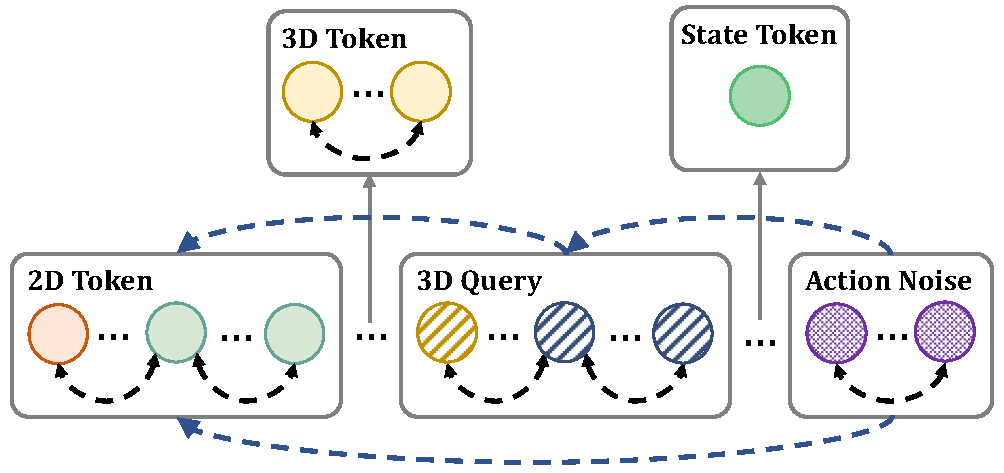
\includegraphics[width=0.47\textwidth]{fig/attention.pdf}
  \caption{\textbf{Block-wise Causal Attention Mechanism.} For simplicity, the detailed attention pathways from the 3D Token and State Token blocks to other blocks are not fully drawn.}
  \label{fig:attention}
  \vspace{-10pt}
\end{figure}


\noindent
\textbf{Training Objective.}
% The model is trained end-to-end with a composite loss function $\mathcal{L}_{total}$, which is a weighted sum of three components:
% We train the entire model end-to-end with a weighted sum of three losses:
% \begin{equation}
%     \mathcal{L}_{total} = \lambda_{1} \mathcal{L}_{action} + \lambda_{2} \mathcal{L}_{track} + \lambda_{3} \mathcal{L}_{depth}
%     \label{eq:total_loss}
% \end{equation}
% Here, $\mathcal{L}_{action}$ is the conditional flow-matching loss from the $\pi_0$ backbone (for continuous action generation), $\mathcal{L}_{track}$ is the keypoint trajectory loss as in Equation~\ref{eq:track_loss}, and $\mathcal{L}_{depth}$ is the depth rendering loss as in Equation~\ref{eq:depth_loss}. The weights $\lambda_{1}$, $\lambda_{2}$, and $\lambda_{3}$ balance the contributions of action, kinematic, and geometric supervision.
%
We train the model end-to-end using a weighted sum of three loss terms:
\vspace{-5pt}
\begin{equation}
    \mathcal{L}_{\text{total}}
    = \lambda_{1}\mathcal{L}_{\text{action}}
    + \lambda_{2}\mathcal{L}_{\text{track}}
    + \lambda_{3}\mathcal{L}_{\text{depth}},
    \label{eq:total_loss}
    \vspace{-5pt}
\end{equation}
where $\mathcal{L}_{\text{action}}$ is the continuous conditional flow-matching loss from $\pi_0$, $\mathcal{L}_{\text{track}}$ is the trajectory prediction loss defined in Eq.~\ref{eq:track_loss}, and $\mathcal{L}_{\text{depth}}$ is the masked depth-rendering loss from Eq.~\ref{eq:depth_loss}. The coefficients $\lambda_{1}$, $\lambda_{2}$, and $\lambda_{3}$ balance supervision from action, kinematic, and geometric signals.



% Here $\mathcal{L}_{action}$ is the conditional flow matching loss from our $\pi_0$ backbone~\cite{black2410pi0}. $\mathcal{L}_{track}$ is the Mean Squared Error loss for the predicted 3D keypoint trajectories, as defined in Equation~\ref{eq:track_loss}. $\mathcal{L}_{depth}$ is the masked L1 loss for the rendered future depth maps, as defined in Equation~\ref{eq:depth_loss}. The terms $\lambda_{1}$, $\lambda_{2}$, and $\lambda_{3}$ are scalar weights that balance each component.

\noindent
\textbf{Inference.}
% During inference, we first feed all context tokens including text, image, history track and 3D query into the LLM Transformer in a \textit{single} forward pass. This pass computes and caches the attention Key-Value pairs for all context and query blocks. The \textbf{action expert} then performs an iterative denoising process for $a$ steps to generate the final action chunk $\textbf{A}_t$. Each of these $a$ steps re-uses the pre-computed KV cache and only requires a forward pass through the much smaller action expert layers~\cite{black2410pi0}.
%
% At inference time, all context tokens—text, images, history track tokens, and 3D queries—are processed by the LLM transformer in a single forward pass, which computes and caches the attention Key–Value pairs for subsequent use. The \textbf{action expert} then performs its iterative denoising procedure for $a$ steps to produce the final action chunk  $\textbf{A}_t$, reusing the cached Key–Value states and invoking only the lightweight action-specific layers.
At inference time, all context tokens including text, images, history track tokens and 3D queries are processed by the transformer in a single forward pass, which computes and caches attention Key--Value pairs for subsequent use. The \emph{action expert} then performs its iterative denoising process for $a$ steps to generate the action chunk $\mathbf{A}_t$, reusing the cached Key--Value states and invoking only its lightweight action-specific layers.

Importantly, the predictive 3D Gaussian geometry modules (e.g., the voxel decoder and depth-rendering module) are not executed during inference. They serve purely as training-time supervision signals that shape the transformer's internal representations with geometric and physical structure, while the action-generation pathway remains unchanged and efficient during deployment.


% Notably, the computationally expensive components for 3D world modeling, such as the Voxel Decoder and the Future Depth Rendering module, are \textbf{not} executed during inference. Their sole purpose during training is to provide a rich and predictive 3D representation on which to condition the action expert, thereby instilling the policy with geometric and physical awareness. This decouples the high-frequency action generation from the complex and non-real-time 3D prediction tasks.
% Crucially, the predictive 3D world-modeling components (e.g., the voxel decoder and depth-rendering module) are not executed during inference. They serve exclusively as training-time supervision mechanisms, shaping the transformer's internal representations with geometric and physical structure while leaving the action-generation phase unchanged and efficient.

\section{Experiments} \label{sec:experiments}
%We conduct extensive experiments to validate the effectiveness of our proposed GeoPredict. Our evaluation is designed to answer several key research questions:

%\begin{enumerate}
    %\item How does GeoPredict perform against our $\pi_0$~\cite{black2410pi0} baseline and other state-of-the-art VLA models on complex long-horizon manipulation benchmarks? We present the corresponding quantitative results on RoboCasa~\cite{nasiriany2024robocasa} and LIBERO~\cite{liu2023libero} benchmarks in Sec.~\ref{sec:main_results}.

    %\item What is the specific contribution of each novel component introduced in our methodology, particularly the trajectory-level kinematic prediction and the predictive 3D Gaussian Splatting world model? We analyze the individual impact of these components through a detailed ablation study in Sec.~\ref{sec:ablations}.

    %\item Does the \textit{Track-based Gaussian Refinement} step measurably improve performance and training efficiency? We investigate this question through quantitative experiments in Sec.~\ref{sec:ablations}, demonstrating its ability to reduce training time while boosting success rates, and provide a visual analysis of the refinement quality in Sec.~\ref{sec:qualitative}.

    %\item How well do the benefits observed in simulation transfer to real-world robotic tasks, especially those demanding precise geometric and spatial reasoning? We report the results on our real-world evaluation suite in Sec.~\ref{sec:real_world}.
%\end{enumerate}

%\noindent We first introduce our experimental setup in Sec.~\ref{sec:exp_setup}.


We first introduce our experimental setup (Sec.~\ref{sec:exp_setup}), followed by a benchmarking against state-of-the-art baselines (Sec.~\ref{sec:main_results}). We then dissect the contribution of our proposed modules through detailed ablation studies (Sec.~\ref{sec:ablations}) and qualitative analysis (Sec.~\ref{sec:qualitative}). Finally, we assess the model's performance in real-world scenarios (Sec.~\ref{sec:real_world}).

\subsection{Experimental Setup} \label{sec:exp_setup}

\noindent \textbf{Simulation Benchmarks.}
We evaluate our method on two widely recognized robotic manipulation benchmarks.
\begin{itemize}[nolistsep, topsep=0pt, itemsep=1pt, parsep=0pt]
    \item \textbf{RoboCasa}~\cite{nasiriany2024robocasa}: This benchmark features 24 complex long-horizon everyday tasks in kitchen environments. We adopt the challenging \texttt{Human-50} few-shot setting, where policies are trained using only 50 human demonstrations per task. To rigorously assess generalization capabilities, we follow the standard protocol by evaluating our model over 50 trials per task across five distinct scenes. This evaluation is conducted exclusively on \textit{unseen object instances}, and includes scenes with \textit{unseen styles} that were never encountered during training.
    
    \item \textbf{LIBERO}~\cite{liu2023libero}: This benchmark is designed to evaluate knowledge transfer and policy generalization across four distinct task suites: LIBERO-Spatial, LIBERO-Object, LIBERO-Goal, and LIBERO-Long. We follow the standard protocol for LIBERO, training policies on 50 human-teleoperated demonstrations for each task and evaluating over 50 trials per task (500 trials per suite).
\end{itemize}


\noindent \textbf{Real-world Evaluation Suite.}
To evaluate GeoPredict's efficacy on real-world tasks requiring precise 3D reasoning, we use an evaluation suite (Figure~\ref{fig:real}). This suite includes three task categories, using 50 expert trajectories per category for training. Each policy is evaluated for 20 trials per category, where success is defined as successfully grasping the target object and placing it in the correct position.

\begin{itemize}[nolistsep, topsep=0pt, itemsep=1pt, parsep=0pt]
    \item \textbf{Spatial Generalization:} The robot is instructed to place the green cube into a plate. We evaluate the policy with the plate located at positions \textit{unseen} during training, testing its ability to generalize to novel target locations.

    \item \textbf{Geometry Generalization:} During the 20 evaluation trials, the model must grasp four distinct object types: a small cube, a medium cube, a large cube, and a rectangular prism. Critically, the test set includes cubes with dimensions \textit{not seen} during training. Furthermore, the rectangular prism is tested in its three unique stable orientations, requiring the policy to adapt its grasp approach based on the perceived object geometry.

    \item \textbf{Visual Robustness:} This task evaluates the policy's resilience to visual distractors. The robot must place the yellow cube into the plate while novel and task-irrelevant objects are introduced into the background of the scene, which were absent during training.
\end{itemize}

\begin{figure}[t]
  \centering
  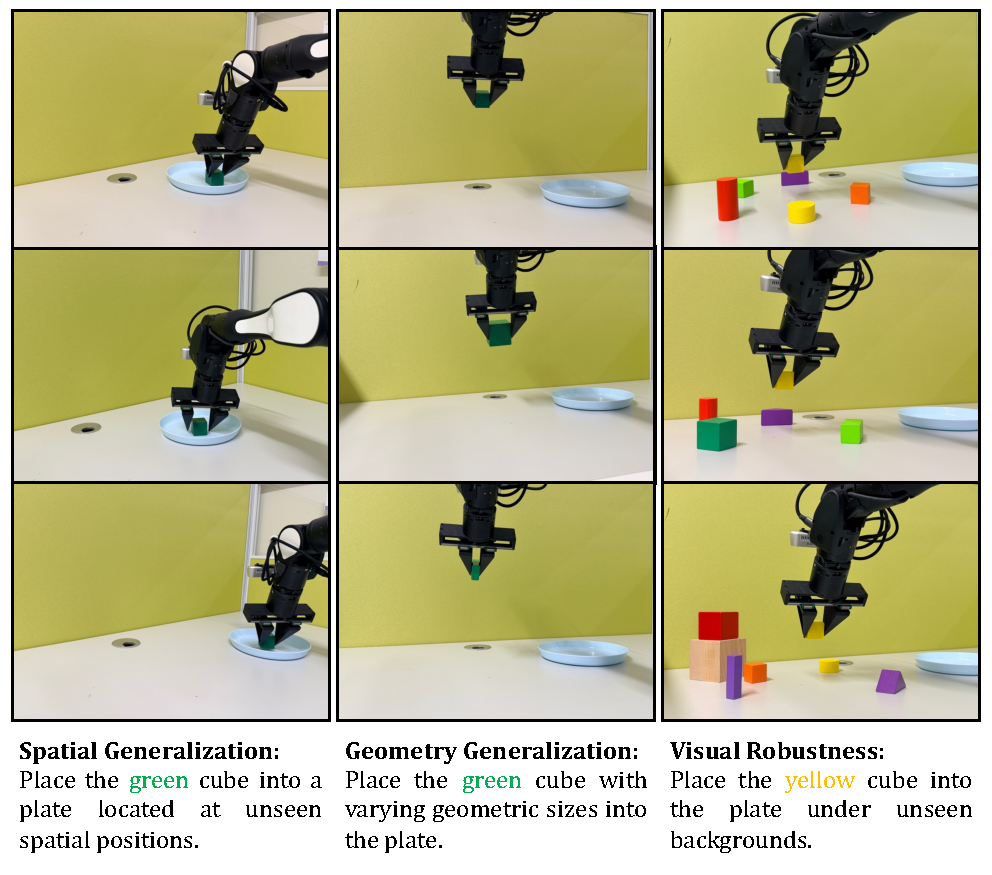
\includegraphics[width=0.47\textwidth]{fig/real.pdf}
  \vspace{-5pt}
  \caption{\textbf{Real-world Evaluation Suite.} These settings aim to evaluate the model's spatial generalization, geometry generalization and robustness to distractors. Each column represents different trials of the same task.}
  \label{fig:real}
  \vspace{-10pt}
\end{figure}

% 多次随机种子得到结果，详细的标准差结果见附录
\begin{table*}[htbp]
\caption{\textbf{RoboCasa Simulation Benchmark Results.} Task success rates (\%) across 24 sub-tasks and the Average Success Rate (\%). $^{\bm{\ast}}$Denotes our fine-tuned experimental results. \textbf{Bold} indicates the best performing model. See Appendix for detailed sub-task definitions.}
\vspace{-5pt}
\centering
\small
\begin{tabular}{l|cccccccccccc} 
\toprule
\multirow{2}{*}{\textbf{Method}} & \textbf{PnP} & \textbf{PnP} & \textbf{PnP} & \textbf{PnP} & \textbf{PnP} & \textbf{PnP} & \textbf{PnP} & \textbf{PnP} & \textbf{CM} & \textbf{CM} & \textbf{CB} & \multirow{2}{*}{\textbf{TSS}} \\
 & \textbf{CTC1} & \textbf{CTC2} & \textbf{CTS1} & \textbf{STC1} & \textbf{CTS2} & \textbf{STC2} & \textbf{CTM} & \textbf{MTC} & \textbf{SU} & S\textbf{V} & \textbf{PS} & \\ 
\midrule

BC-Transformer~\cite{nasiriany2024robocasa}& 6.0 & 2.0 & 2.0 & 8.0 & 2.0 & 6.0 & 2.0 & 2.0 & 0.0 & 22.0 & 48.0 & 54.0 \\

GWM~\cite{lu2025gwm} & 4.0 & \textbf{18.0} & 20.0 & 22.0 & 2.0 & 18.0 & 14.0 & \textbf{20.0} & 16.0 & 36.0 & \textbf{76.0} & \textbf{72.0} \\

$\pi_0^{\bm{\ast}}$ (Baseline)~\cite{black2410pi0} & 24.0 & 6.8 & 26.8 & 15.6 & 11.2 & 12.8 & 6.8 & 7.6 & 18.4 & 33.6 & 74.0 & 69.6 \\

\textbf{GeoPredict (Ours)} & \textbf{32.4} & 8.8 & \textbf{27.6} & \textbf{31.2} & \textbf{20.4} & \textbf{28.8} & \textbf{14.4} & 18.0 & \textbf{28.4} & \textbf{49.2} & 67.6 & 70.8 \\

\midrule
\textbf{Average Success Rate} & 
\textbf{OSD} &
\textbf{CSD} &
\textbf{ODD} &
\textbf{CDD} &
\textbf{OD} &
\textbf{CD} &
\textbf{TNSF} &
\textbf{TFSF} &
\textbf{TNS} &
\textbf{TFS} &
\textbf{TNM} &
\textbf{TFM} \\
\midrule

\multicolumn{1}{c|}{28.8} & 46.0 & 56.0 & 28.0 & 28.0 & 42.0 & 80.0 & 38.0 & 50.0 & 32.0 & 4.0 & 62.0 & 70.0\\

\multicolumn{1}{c|}{39.2} & \textbf{58.0} & 54.0 & 28.0 & 50.0 & 56.0 & 80.0 & 52.0 & 44.0 & 46.0 & \textbf{22.0} & 64.0 & 70.0\\

\multicolumn{1}{c|}{42.3} & 40.8 & \textbf{82.0} & 55.2 & 69.2 & 66.4 & 96.0 & 43.6 & 86.0 & 43.2 & 6.0 & 59.6 & 60.0\\

\multicolumn{1}{c|}{\textbf{52.4}} & 40.4 & 78.8 & \textbf{87.2} & \textbf{70.0} & \textbf{77.6} & \textbf{96.8} & \textbf{72.4} & \textbf{94.8} & \textbf{60.0} & 13.2 & \textbf{84.8} & \textbf{82.8}\\

\bottomrule
\end{tabular}
\label{tab:robocasa}
\vspace{-5pt}
\end{table*}




\begin{table*}[htbp]
\centering
\small
\caption{\textbf{LIBERO Simulation Benchmark Results.} Task success rates (\%) across 4 evaluation suites and the Average Success Rate (\%). $^{\bm{\ast}}$Denotes our reproduced experimental results. $^{\bm{\dagger}}$Denotes no available standard deviation data. \textbf{Bold} indicates the \textbf{best} performing model, and \underline{underline} indicates the \textbf{runner-up} model.}
\vspace{-5pt}
\begin{tabular}{l | c  c  c  c | c}
\toprule
\textbf{Method} & 
\multicolumn{1}{c}{\textbf{LIBERO-Spatial}} & 
\multicolumn{1}{c}{\textbf{LIBERO-Object}} & 
\multicolumn{1}{c}{\textbf{LIBERO-Goal}} & 
\multicolumn{1}{c|}{\textbf{LIBERO-Long}} & 
\multicolumn{1}{c}{\textbf{Average}} \\
\midrule
Diffusion Policy~\cite{chi2025diffusion} & 78.3 $\pm$ 1.1 & 92.5 $\pm$ 0.7 & 68.3 $\pm$ 1.2 & 50.5 $\pm$ 1.3 & 72.4 $\pm$ 0.7 \\
TraceVLA~\cite{zheng2024tracevla} & 84.6 $\pm$ 0.2 & 85.2 $\pm$ 0.4 & 75.1 $\pm$ 0.3 & 54.1 $\pm$ 1.0 & 74.8 $\pm$ 0.5 \\
Octo~\cite{team2024octo} & 78.9 $\pm$ 1.0 & 85.7 $\pm$ 0.9 & 84.6 $\pm$ 0.9 & 51.1 $\pm$ 1.3 & 75.1 $\pm$ 0.6 \\
OpenVLA~\cite{kim2025openvla} & 84.7 $\pm$ 0.9 & 88.4 $\pm$ 0.8 & 79.2 $\pm$ 1.0 & 53.7 $\pm$ 1.3 & 76.5 $\pm$ 0.6 \\
SpatialVLA~\cite{qu2025spatialvla} & 88.2 $\pm$ 0.5 & 89.9 $\pm$ 0.7 & 78.6 $\pm$ 0.6 & 55.5 $\pm$ 1.0 & 78.1 $\pm$ 0.7 \\
WorldVLA$^{\bm{\dagger}}$~\cite{cen2025worldvla} & 87.6 & 96.2 & 83.4 & 60.0 & 81.8 \\
4D-VLA~\cite{zhang20254d} & 88.9 $\pm$ 0.5 & 95.2 $\pm$ 0.3 & 90.9 $\pm$ 0.4 & 79.1 $\pm$ 1.2 & 88.6 $\pm$ 0.3 \\
DreamVLA$^{\bm{\dagger}}$~\cite{zhangdreamvla} & \underline{97.5} & 94.0 & 89.5 & 89.5 & 92.6 \\
$\pi_0^{\bm{\dagger}}$~\cite{black2410pi0} & 96.8 & \textbf{98.8} & \textbf{95.8} & 85.2 & 94.2\\
OpenVLA-OFT$^{\bm{\dagger}}$~\cite{kim2025fine} & 95.2 & 94.2 & 95.2 & \underline{93.2} & 94.5 \\
UniVLA$^{\bm{\dagger}}$~\cite{bu2025univla} & 96.5 & 96.8 & 95.6 & 92.0 & \underline{95.2} \\
\midrule
$\pi_0^{\bm{\ast}}$ (Baseline)~\cite{black2410pi0} & 96.6 $\pm$ 0.6 & 97.2 $\pm$ 0.8 & 94.2 $\pm$ 0.7 & 87.6 $\pm$ 1.1 & 93.9 $\pm$ 0.4\\
\textbf{GeoPredict (Ours)} & \textbf{98.0 $\pm$ 0.7} & \underline{98.2 $\pm$ 0.7} & \underline{95.7 $\pm$ 0.2} & \textbf{94.0 $\pm$ 1.0} & \textbf{96.5 $\pm$ 0.6} \\
\bottomrule
\end{tabular}
\label{tab:libero}
\vspace{-10pt}
\end{table*}

\noindent \textbf{Baselines.}
Our primary baseline is our VLA backbone, \textbf{$\pi_0$}~\cite{black2410pi0}, trained without our proposed predictive 3D modules. This comparison directly isolates the contribution of our geometry-aware predictive method. We also compare against a range of state-of-the-art VLA and world-modeling approaches, including BC-Transformer~\cite{nasiriany2024robocasa}, GWM~\cite{lu2025gwm}, OpenVLA~\cite{kim2025openvla}, SpatialVLA~\cite{qu2025spatialvla} and UniVLA~\cite{bu2025univla}.


\noindent \textbf{Implementation Details.}
A predictive horizon of $H=50$ is used for all tasks. Observations include two environment and one wrist camera views. Depth supervision is applied only to the two $224\times224$ environment cameras. For the trajectory-level prediction module (Sec.~\ref{sec:track_query}), we track $K=8$ keypoints (7 joints, 1 end-effector) for LIBERO~\cite{liu2023libero} and RoboCasa~\cite{nasiriany2024robocasa}, and $K=7$ (6 joints, 1 end-effector) for the real-world setup. For the predictive 3DGS geometry module (Sec.~\ref{sec:3dgs}), the workspace is $1.6\text{m} \times 1.6\text{m} \times 1.0\text{m}$ with $v=0.04$m voxels. Token and decoder feature dimensions are $C=2048$ and $C'=256$. We use $N_G=4$ initial primitives per voxel, and generate $N_G'=64$ additional primitives for voxels selected by the track-guided refinement mechanism. All loss weights in Eq.~\eqref{eq:total_loss} are 1.0. We train for 40,000 iterations using AdamW~\cite{loshchilovdecoupled} (LR 2.5e-5) on 8 NVIDIA H20 GPUs with a total batch size of 32. The primary metric is Task Success Rate (\%).










\subsection{Main Results} \label{sec:main_results}

\noindent \textbf{RoboCasa.}
Table~\ref{tab:robocasa} details the performance across the 24 RoboCasa sub-tasks. GeoPredict achieves an average success rate of \textbf{52.4\%}, significantly outperforming all baselines. Notably, it improves upon the $\pi_0$ baseline success rate of 42.3\% by a margin of \textbf{10.1\%}. This substantial gain underscores the benefit of conditioning the policy on predictive kinematic and geometric priors, especially in the \texttt{Human-50} few-shot setting where generalization from limited data is critical~\cite{nasiriany2024robocasa}. Moreover, GeoPredict demonstrates clear advantages over other future prediction methods such as GWM~\cite{lu2025gwm} at 39.2\% and 2D policies like BC-Transformer~\cite{nasiriany2024robocasa} at 28.8\%. Additional large-scale results on RoboCasa \texttt{Generated-300} are in the Appendix.




\noindent \textbf{LIBERO.}
In Table~\ref{tab:libero}, we show results on the four LIBERO suites~\cite{liu2023libero}. GeoPredict achieves an average success rate of \textbf{96.5\%}, surpassing the current SOTA method UniVLA~\cite{bu2025univla}. Furthermore, it significantly outperforms strong baselines such as OpenVLA~\cite{kim2025openvla} which attains 76.5\% by a margin of 20.0\%. Our model demonstrates consistently high performance across all four suites, including Spatial (98.0\%), Object (98.2\%), Goal (95.7\%), and the challenging Long (94.0\%). This indicates that our method's geometry-aware training is highly effective and generalizes robustly across diverse tasks and environments.


\subsection{Ablation Study} \label{sec:ablations}
\noindent \textbf{Component Ablation.}
Table~\ref{tab:ab_module} details our ablation, building the model from the ground up. Starting from the $\pi_0$ baseline (42.3\%), adding the history Track Encoder provides a kinematic prior, improving performance to 44.8\%. Adding the Future Track Query ($\mathcal{L}_{track}$) for explicit motion prediction further boosts the rate to 47.2\%.

The predictive 3D Gaussian Splatting geometry module yields the most substantial gains. Supervising with $\mathcal{L}_{depth}$ (using only initial $\mathbf{G}^{init}$) elevates performance to 49.4\%. Jointly training with $\mathcal{L}_{track}$ and $\mathcal{L}_{depth}$ but without the explicit \textit{track-guided refinement} yields 50.5\%. Critically, activating the full \textit{track-guided refinement} mechanism, which allocates geometric capacity along the predicted future tracks, achieves the peak 52.4\%. This final 1.9\% gain (50.5\% $\to$ 52.4\%) validates our hypothesis: using kinematic predictions to refine the 3DGS representation provides a superior geometric prior for the policy.

\noindent \textbf{Ablation on Depth Rendering.}
Table~\ref{tab:ab_depth} ablates our predictive 3DGS method. Rendering with color (49.2\%) offers no benefit over depth-only (49.4\%), confirming geometric information alone suffices. Increasing the global initial primitives from $N_G=4$ to $N_G=8$ (51.4\%) significantly increases training time (12.0 to 19.1 hours/epoch).

In contrast, our \textit{track-guided refinement} strategy ($N_G=4, N_G'=8$) is more efficient, achieving 51.1\% at only 15.5 hours/epoch. This highlights the efficiency of allocating geometric capacity to task-relevant interaction regions. Since these regions are a small fraction of the volume, we can increase $N_G'$ with negligible overhead. Setting $N_G'=64$ yields our peak 52.4\% success rate at a near-identical 15.7 hours. Therefore, we adopt $N_G=4$ and $N_G'=64$ as our final configuration.

\begin{table}[t]
\centering
\small
\caption{\textbf{Ablation Study on RoboCasa Simulation Benchmark.} Future Depth is rendered from initial global Gaussians ($\textbf{G}^{init}$), while Future Depth$^{\bm{\ast}}$ utilizes the refined total Gaussians ($\textbf{G}^{total}$). Results denote the Average Success Rate (\%) across all sub-tasks.}
\vspace{-5pt}
\begin{tabular}{l | c  c  c  c c c}
\toprule
History Track & \textcolor{red}{\ding{56}} & \textcolor{blue}{\ding{52}} & \textcolor{blue}{\ding{52}} & \textcolor{red}{\ding{56}} & \textcolor{blue}{\ding{52}} & \textcolor{blue}{\ding{52}}\\
Future Track & \textcolor{red}{\ding{56}} & \textcolor{red}{\ding{56}} & \textcolor{blue}{\ding{52}} & \textcolor{red}{\ding{56}} & \textcolor{blue}{\ding{52}} & \textcolor{blue}{\ding{52}}\\
Future Depth & \textcolor{red}{\ding{56}} & \textcolor{red}{\ding{56}} & \textcolor{red}{\ding{56}} & \textcolor{blue}{\ding{52}} & \textcolor{blue}{\ding{52}} & \textcolor{red}{\ding{56}}\\
Future Depth$^{\bm{\ast}}$ & \textcolor{red}{\ding{56}} & \textcolor{red}{\ding{56}} & \textcolor{red}{\ding{56}} & \textcolor{red}{\ding{56}} & \textcolor{red}{\ding{56}} & \textcolor{blue}{\ding{52}}\\
\midrule
\textbf{Average SR} & 42.3 & 44.8 & 47.2 & 49.4 & 50.5 & 52.4\\
\bottomrule
\end{tabular}
\label{tab:ab_module}
\vspace{-3pt}
\end{table}



\begin{table}[t]
\centering
\small
\caption{\textbf{Ablation Study on Depth Rendering.} $N_G$ and $N_G'$ denote the number of Gaussian primitives per voxel for the initial and refined stages, respectively. Color indicates RGB image reconstruction. \textbf{Time / Epoch} represents the training time per epoch in hours, and \textbf{Average SR} is the Average Success Rate (\%).}
\vspace{-5pt}
\begin{tabular}{l | c  c  c  c c c}
\toprule
$N_G$ & 4 & 4 & 8 & 4 & 4 \\
$N_G'$ & \textcolor{red}{\ding{56}} & \textcolor{red}{\ding{56}} & \textcolor{red}{\ding{56}} & 8 & 64 \\
Color & \textcolor{blue}{\ding{52}} & \textcolor{red}{\ding{56}} & \textcolor{red}{\ding{56}} & \textcolor{red}{\ding{56}} & \textcolor{red}{\ding{56}} \\
\midrule
\textbf{Time / Epoch} & 12.3 & 12.0 & 19.1 & 15.5 & 15.7 \\
\textbf{Average SR} & 49.2 & 49.4 & 51.4 & 51.1 & 52.4\\
\bottomrule
\end{tabular}
\label{tab:ab_depth}
\vspace{-3pt}
\end{table}

\subsection{Qualitative Analysis} \label{sec:qualitative}
Figure~\ref{fig:vis} provides a qualitative visualization of our predictive 3DGS geometry module, which compares the predicted future depths at various timesteps ($t+1, t+10, t+20$). While the \textbf{initial} Gaussians ($\mathbf{G}^{init}$) capture only the coarse scene layout, the \textbf{refined} Gaussians ($\mathbf{G}^{total}$) exhibit significantly sharper geometric details, particularly surrounding the robotic arm. This visually confirms that our refinement mechanism produces a more precise and geometrically-faithful prediction of the future, which in turn provides a superior conditional prior for the action expert.

\begin{figure}[t]
  \centering
  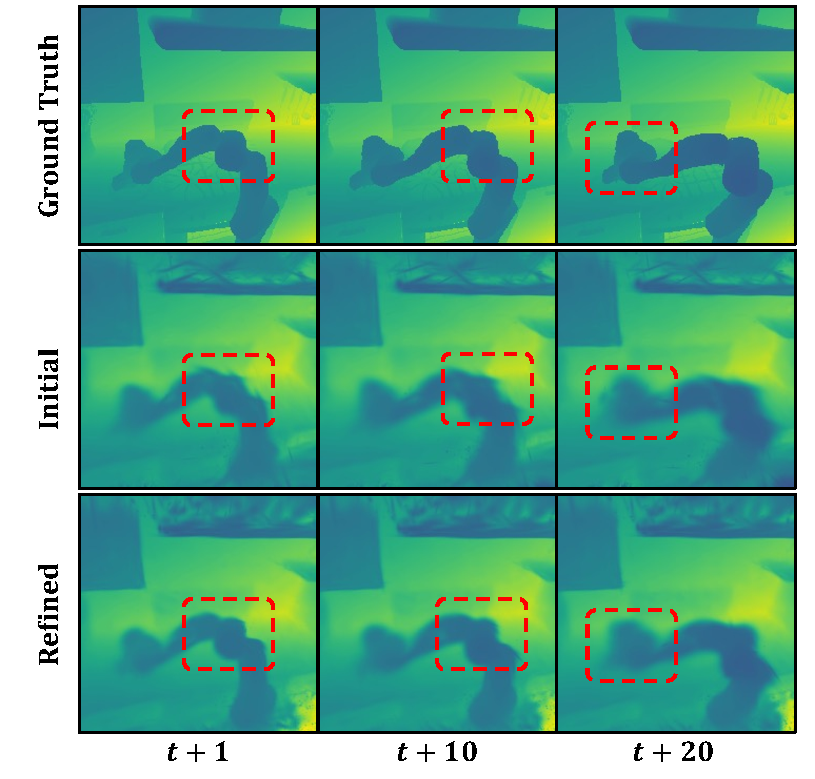
\includegraphics[width=0.47\textwidth]{fig/vis.pdf}
  \vspace{-5pt}
  \caption{\textbf{Qualitative Comparisons of Future Depth Rendering.} Visualizations are shown for timesteps $t+1, t+10, \text{and } t+20$. \textcolor{red}{Red boxes} highlight the improvements in fine-grained geometric details. Best viewed zoomed in.}
  \vspace{-10pt}
  \label{fig:vis}
\end{figure}



\begin{table}[t]
\centering
\small
\caption{\textbf{Real-World Experiment Results.} Task success rates (\%) across three distinct settings: Spatial, Geometry, and Robustness.}
\vspace{-5pt}
\begin{tabular}{l | c c c}
\toprule
\textbf{Method} & \textbf{Spatial} & \textbf{Geometry} & \textbf{Robustness}\\
\midrule
$\pi_0$ (Baseline)~\cite{black2410pi0} & 60.0 & 50.0 & 35.0  \\
\textbf{GeoPredict (Ours)} & 85.0 & 95.0 & 90.0 \\
\bottomrule
\end{tabular}
\label{tab:real}
\vspace{-7pt}
\end{table}


\subsection{Real-World Experiments} \label{sec:real_world}
We validate GeoPredict on a DISCOVER robotic arm to assess performance on tasks demanding explicit 3D reasoning. As detailed in Table~\ref{tab:real}, GeoPredict significantly outperforms the $\pi_0$~\cite{black2410pi0} baseline across all tasks. Specifically, in the Spatial and Robustness tasks, our method achieves success rates of 85.0\% and 90.0\% respectively, surpassing the baseline scores of 60.0\% and 35.0\% and demonstrating superior spatial generalization and resilience to distractors. In the Geometry task, GeoPredict attains a 95.0\% success rate compared to 50.0\% for the baseline. This 45.0\% improvement on tasks involving object sizes absent from the training set strongly indicates that our predictive 3DGS module endows the policy with a generalizable understanding of 3D geometry, enabling adaptive grasping capabilities that the 2D-centric $\pi_0$ baseline lacks. Moreover, since our method explicitly encodes motion history via the Track Encoder, the Appendix provides a dedicated real-world experiment to validate the effectiveness of this historical context.

\section{Conclusion}
\label{sec:conclusion}
% We presented \textbf{GeoPredict}, a geometry-aware VLA framework that augments a continuous-action policy with predictive kinematic and geometric priors. By jointly learning future robot keypoint trajectories and future workspace geometry via a predictive 3D Gaussian Splatting model with track-guided refinement, GeoPredict provides the transformer with future-aware structure while keeping inference lightweight. Extensive experiments on simulation and real-world manipulation tasks show that GeoPredict consistently improves over strong VLA baselines, particularly in settings that demand precise 3D reasoning, geometric robustness, and long-horizon physical consistency. We believe this training-time predictive supervision offers a promising direction for building more reliable and geometry-aware VLA controllers.

We presented \textbf{GeoPredict}, a geometry-aware VLA framework enhancing continuous-action policies with predictive kinematic and geometric priors. By forecasting robot trajectories and workspace geometry via track-guided 3DGS, GeoPredict introduces future-aware structure into the transformer while keeping inference lightweight. Extensive experiments show consistent superiority over strong baselines in tasks requiring precise 3D reasoning, geometric robustness and long-horizon physical consistency. While acquiring multi-view RGB-D and camera extrinsics presents scaling challenges, the increasing availability of calibrated depth in modern datasets and commodity hardware mitigates these concerns. Ultimately, our training-time predictive supervision provides a promising direction for reliable, geometry-aware, and grounded VLA controllers.



\section*{Acknowledgment}
{\sloppy
This work is supported by the Shenzhen Science and Technology Program (Grant No. ZDCY20250901113000001) and the 1+1+1 CUHK-CUHK(SZ)-GDSTC Joint Collaboration Fund (Grant No. 2025A0505000079). We gratefully acknowledge DISCOVER Robotics for providing hardware support.
\par}

{
    \small
    \bibliographystyle{ieeenat_fullname}
    \bibliography{main}
}

% WARNING: do not forget to delete the supplementary pages from your submission 
% \input{sec/X_suppl}

\end{document}
